\documentclass[11pt]{article}

\usepackage[utf8]{inputenc}
\usepackage{amsmath, amssymb, amsthm}
\usepackage[inkscapeformat=pdf]{svg}
\usepackage{placeins}
\usepackage{tabularx}
\usepackage{float}
\usepackage{setspace}
\usepackage{hyperref}
\usepackage{enumitem}
\usepackage{parskip}
\usepackage{ffcode}
\usepackage{graphicx}

\usepackage[margin=2cm]{geometry}

\def\code#1{{\texttt{#1}}}

\title{%
  \textbf{RASD} \\
  \large Software Engineering Project \\ A.Y. 2022-2023}

\author{Marco Ronzani, Alessandro Sassi}

\date{November 2022}

\begin{document}

\maketitle

\doublespacing
\tableofcontents
\singlespacing

\section{Introduction}
\label{section:introduction}

\subsection{Purpose}

Electric vehicles are starting to grow in number, and their takeover of combustion engines is bound to happen, consequently to support such a thriving trend adequate easy access to charging stations is of utmost importance. In this landscape the goal of eMall is to allow owners of electric vehicles to easily know where charging stations are and carefully plan their charging process according to their schedules at any such station.\\
\\
This document will discuss goals and requirements that regard the system necessary to make eMall a reality, with the purpose of guiding the development process.

%Description of the System To Be:
%It is composed of the eMSP and one or more CPMSs ... description
%=> CPMS non va condiserato come actor perchè parte del STB

%Actor: User, DSO, CPO

%Consideration:
%CPMSs are not necessarily part of eMall, they might be entirely separated and can be reasonably assumed to exist independently.

%A CS has associated a DSO (one exactly at every instant) and is "plugged" thanks to it in the electric grid. The management of batteries is also handled per-CS.

%The user is charged a price that is exactly the energy he used times the original price he booked the CS for, hence eventual changes operated by the CPMS during the process that alter the cost of electricity do not affect the user's charge, simply the difference kept or given by the CPO/CPMS.

%A user should be able to show up whenever at a free socket and charge by "booking it on the fly" for the time window the socket is free!

%Machine: eMSPs + CPMSs
%World: Users + CS (charging stations) + Sockets + DSOs + CPOs

\subsubsection{Goals}

\begin{table}[H]
    \centering
    %space between text and right/left borders
    \setlength{\tabcolsep}{18pt}
    %Row height multiplier
    \renewcommand{\arraystretch}{1.2}
    \begin{tabularx}{\textwidth}{|>{\centering\hsize=0.3\hsize}X|>{\hsize=1.7\hsize}X|}
        \hline
        \textbf{Goal} & \textbf{Description} \\
        \hline
        G1 & Allow Users to see the list of available Charging Stations \\
        \hline
        G2 & Allow Users to see the cost of a recharge and special offers for a Charging Station \\
        \hline
        G3 & Allow Users to book charging time slots \\
        \hline
        G4 & Allow Users to monitor, manage and pay for their booked charging sessions \\
        \hline
        %G5 & Allow Charge Point Operators to manage the provider each Charging Station uses to source energy \\
        G5 & Allow Charge Point Operators to manage the energy sources each Charging Station uses \\
        \hline
    \end{tabularx}
    \label{tab:goals}
\end{table}

\subsection{Definitions, Acronyms and Abbreviations}

\subsubsection{Definitions}

\begin{table}[H]
    \centering
    %space between text and right/left borders
    \setlength{\tabcolsep}{18pt}
    %Row height multiplier
    \renewcommand{\arraystretch}{1.2}
    \begin{tabularx}{\textwidth}{|>{\centering\hsize=0.4\hsize}X|>{\hsize=1.6\hsize}X|}
        \hline
        \textbf{Term} & \textbf{Definition} \\
        \hline
        Charging Station & Device with a connection to the electric grid which brakes out power to one or more socket(s) for vehicles. Monitoring of each socket's status. \\
        \hline
        Charging Session & The process in which a User performs a recharge of their vehicle. \\
        \hline
        Energy source of a Charging Station & Batteries or the DSO currently assigned to the CS, whichever the CS is currently drawing its power from. \\
        \hline
        Charging Station External Status & Number of charging sockets available, their type such as slow/fast/rapid, their cost, and, if all sockets of a certain type are occupied, the estimated amount of time until the first socket of that type is freed. \\
        \hline
        Charging Station Internal Status & Amount of energy available in the batteries, if any, number of vehicles being charged and, for each charging vehicle, amount of power absorbed and time left to the end of the recharge. \\
        \hline
        Energy Source & Method of energy production that results in a known fraction of the energy supplied to an endpoint in the electric grip. \\
        \hline
        User-price & Cost of a recharge that is shown to the User when they inspect a CS and is what they are charged for. It is set by the CPO/CPMS on a per-CS basis.\\
        \hline
        Nominal-price & Cost of a recharge at a CS without any discount or offer applied, it is set by the CPO/CPMS. A user-price $<$ nominal-price implies an ongoing special offer. \\
        \hline
        Energy source management policy OR Battery usage policy & The global policy used by the CPMS to dynamically decide for each CS its energy source or if ts should start charging its batteries. \\
        \hline
    \end{tabularx}
    \label{tab:definitions}
\end{table}

\subsubsection{Acronyms}

\begin{table}[H]
    \centering
    %space between text and right/left borders
    \setlength{\tabcolsep}{18pt}
    %Row height multiplier
    \renewcommand{\arraystretch}{1.2}
    \begin{tabularx}{\textwidth}{|>{\centering\hsize=0.3\hsize}X|>{\hsize=1.7\hsize}X|}
        \hline
        \textbf{Acronym} & \textbf{Full Name} \\
        \hline
        eMall & Electric Mobility for All \\
        \hline
        eMSP & Electric Mobility Service Provider \\
        \hline
        CPO & Charging Point Operator \\
        \hline
        CPMS & Charge Point Management System \\
        \hline
        CS & Charging Station \\
        \hline
        DSO & Distribution System Operator \\
        \hline
        STB & System-To-Be \\
        \hline
        OS & Operating system \\
        \hline
    \end{tabularx}
    \label{tab:acronyms}
\end{table}

\subsection{Scope}

This RASD document takes into consideration the requirements and specifications of the eMSP platform “eMall”, together with its interaction with one or more CPMSs. The stakeholders considered are the End Users who interact with the “eMall” platform, CPOs owning the respective CSs and CPMSs, and DSOs offering their services to the aforementioned parties.

\subsubsection{World Phenomena}

\begin{table}[H]
    \centering
    %space between text and right/left borders
    \setlength{\tabcolsep}{18pt}
    %Row height multiplier
    \renewcommand{\arraystretch}{1.2}
    \begin{tabularx}{\textwidth}{|>{\centering\hsize=0.3\hsize}X|>{\hsize=1.7\hsize}X|}
        \hline
        \textbf{Phenomena} & \textbf{Description} \\
        \hline
        WP1 & Electric vehicles connect to a CS socket \\
        \hline
        WP2 & CPOs add/remove available CSs \\
        \hline
        %DOMAIN ASSUMPTION: If you change sockets you change tho whole CS!
        WP3 & CPOs add/remove batteries from existing CSs \\
        \hline
        WP4 & CPOs decide the policy with which to assign DSOs to CSs \\
        \hline
        WP5 & DSOs set the price and/or the mix of sources for the electricity they provide \\
        \hline
        WP6 & CPOs pay DSOs for the consumed electricity \\
        \hline
    \end{tabularx}
    \label{tab:world_phenomena}
\end{table}

\subsubsection{Shared Phenomena}

In order to represent more clearly whether a phenomenon is world or machine controlled or observed, we define a list of acronyms used only for the scope of the Shared Phenomena definition. These acronyms will also be reported in the Shared Phenomena table, so that for each entry the controller/observer party can easily be identified. 

\begin{table}[H]
    \centering
    %space between text and right/left borders
    \setlength{\tabcolsep}{18pt}
    %Row height multiplier
    \renewcommand{\arraystretch}{1.2}
    \begin{tabularx}{\textwidth}{|>{\centering\hsize=0.3\hsize}X|>{\hsize=1.7\hsize}X|}
        \hline
        \textbf{Type} & \textbf{Explanation} \\
        \hline
        MO & Machine Observed Phenomenon, the STB takes notice of the event \\
        \hline
        MC & Machine Controlled Phenomenon, the STB causes the event \\
        \hline
        WO & World Controlled Phenomenon, an/some external agent(s) notices the event \\
        \hline
        WC & World Controlled Phenomenon, an/some external agent(s) causes the event \\
        \hline
    \end{tabularx}
    \label{tab:shared_phenomena_header}
\end{table}

\begin{table}[H]
    \centering
    %space between text and right/left borders
    \setlength{\tabcolsep}{18pt}
    %Row height multiplier
    \renewcommand{\arraystretch}{1.2}
    \begin{tabularx}{\textwidth}{|>{\centering\hsize=0.3\hsize}X|>{\centering\hsize=0.3\hsize}X|>{\hsize=1.4\hsize}X|}
        \hline
        \textbf{Phenomena} & \textbf{Type} & \textbf{Description} \\
        \hline
        SP1 & WC MO & The User views the available charging stations and their information \\
        \hline
        SP2 & WC MO & Users book a charging session to a CS \\
        \hline
        SP3 & WC MO & Users start their vehicle's charging session on a CS \\
        \hline
        SP4 & MC WO & The eMSP notifies users of the completion of their vehicle's charging session \\
        \hline
        SP5 & WC MO & Users prematurely terminate their ongoing charging session \\
        \hline
        SP6 & WC MO & Users are charged for their finished charging sessions \\
        \hline
        %Since CPOs need those to manually manage CSs!!
        SP7 & MC WO & CPMSs publish the location and external status information regarding their managed CSs \\
        \hline
        %There are two energy prices, the one the DSOs charge the CPOs for and the one the CPOs charge the Users for!
        SP8 & WC MO & CPOs update the DSO associated to a CS (this determines how much a CPO is charged for the electricity a CS provides) \\
        \hline
        SP9 & WC MO & CPOs update the user-price of energy and set special offers for a CS \\
        \hline
        %SP10 & WC MO & CPOs perform an addition/removal of CSs \\
        %\hline
        SP10 & WC MO & CPOs update batteries information and batteries usage policies for their CSs \\
        \hline
        SP11 & MC WO & The eMSP transfers the amount due to CPOs for performed recharges \\
        \hline
    \end{tabularx}
    \label{tab:shared_phenomena}
\end{table}

\subsection{Revision History}

\begin{enumerate}
    \item[v0.1] First draft of the document.
\end{enumerate}

\subsection{Reference Documents}

\begin{enumerate}
    \item The provided document describing the project: \textit{Assignment RDD AY 2022-2023-v3}.
    \item The Software Engineering 2 course held by Prof.s Camilli Matteo, Di Nitto Elisabetta and Rossi Matteo Giovanni.
    \item \textit{ISO/IEC/IEEE 29148:2011(E)} standard for Requirement Engineering.
    \item Project of last year provided as an assignment.
\end{enumerate}

\subsection{Document Structure}

This document is based on the \textit{ISO/IEC/IEEE 29148:2011(E)} document and adheres to the requirements analysis procedures of \textit{ISO/IEC 12207}. The document is divided into the following six sections. \\
\\
The \hyperref[section:introduction]{\textbf{introduction}} informally introduces the scope and purpose of the STB this document analyses, following up such description with a formal elicitation of goals and phenomena that together provide a characterization of the world around the STB and what will the STB bring to such environment. In this section useful information to read the document is provided as well, such as acronyms, the document's revision history and other referenced documents. \\
\\
The \hyperref[section:overallDescription]{\textbf{overall description}} follows with detailed modelling of the world around the STB and the scenarion in which the system will be interacting with all the different external users. This section identifies and describes the uses of the system and the functions the STB will offer, as well as posing the needed domain assumptions to supplement the current model. \\
\\
The \hyperref[section:specificRequirements]{\textbf{specific requirements}} section focuses on functional and non functional requirements, starting from the interfaces of the system towards external entities and other system elements, following with a formal elicitation of functional requirements and their contextualization with goals and domain assumptions. Finally design constraints and software system attributes are described in this section to complement requirements. \\
\\
Follows the \hyperref[section:alloy]{\textbf{formal analysis using Alloy}} which presents the Alloy code related to the described model and the results provided by its usage. \\
\\
The \hyperref[section:effort]{\textbf{effort spent}} section presents data regarding the amount of time each team member invested in the creation of this document. \\
\\
Finally \hyperref[section:references]{\textbf{references}} are reported.

\newpage

\section{Overall Description}
\label{section:overallDescription}

\subsection{Product Perspective}

\subsubsection{Scenarios}
\label{subsubsec:scenarios}

\begin{description}
    \item [1. New user registration] \hfill \\
        \textit{Actors: Unregistered User} \\
        A person, Bob, who discovered eMall has decided to register into the platform to use its recharge booking and recharge management system. To this end Bob reaches the eMall services and chooses to “sign up”, after that Bob fills in the relevant information and his eMall account is created. Now Bob can proceed to login.
    \item [2. User login] \hfill \\
        \textit{Actors: Registered User} \\
        An already registered user, Bob, reaches the eMall services and intends to either book a charging spot or to manage a currently ongoing recharge booked to his name, hence Bob chooses to “login” and enters its credentials. Assuming Bob inserted valid credentials he now has a valid session within the eMall services. If Bob failed in setting valid credentials he can try again.
    \item [3. User looking for charging stations] \hfill \\
        \label{scenario:lookingForCS}
        \textit{Actors: Registered User} \\
        A user already registered on eMall, Bob, needs to know the location and/or pricing of CSs in a certain are of his interest. To obtain such data, Bob has reached the eMall services, has logged in and has selected the charging stations “search” options. Now Bob can search for CSs and is presented with multiple filters to control:
        \begin{itemize}
            \item His area of interest
            \item Recharge price ranges
            \item Connector types available
            \item Charging speeds available
        \end{itemize}
        By manipulating the filters Bob can restrict or widen the scope of his search. Results of the search are displayed in respect of the filters and Bob can see the details of every result such as:
        \begin{itemize}
            \item Location
            \item Price
            \item Offers
            \item Booking schedule
            \item Available connectors
            \item Available charging speeds
        \end{itemize}
    \item [4. User booking a recharge] \hfill \\
        \textit{Actors: Logged-in User} \\
        A user Bob has already performed the login and now intends to book a recharge. Bob first performs a search for the CS to reserve for his recharge (see “user looking for charging stations” scenario) and once he finds a suitable and available one chooses “book recharge” for that station. Bob is then presented with the choice for the time slot for his recharge and once he chooses his reservation is completed.
    \item [5. User deleting one of his bookings] \hfill \\
        \textit{Actors: Logged-in User} \\
        A user Bob has already performed the login and recently made a few bookings on eMall. However on second thought Bob realized he could not make it in time for one of his bookings and now intends to delete it. To this end Bob selects the option to view his meetings' list on eMall and selects the meeting he desires to remove, he chooses the delete option the meeting list is updated with the deleted meeting now missing, confirming that eMall discarded it.
    \item [6. User performing a charging process (start, monitor and pay)] \hfill \\
        \textit{Actors: Logged-in User} \\
        The user Bob has previously booked a recharge at a certain CS for a certain time slot. Bob shows up at the CS during his reserved time slot and proceeds to connect his vehicle properly. Once the vehicle is connected Bob reaches the eMall services to start the charging process. After the process is started Bob has the option to interrupt it at any time, otherwise the charging procedure automatically halts as the CS noticed the vehicle’s battery being full or the booked time slot expires. Bob is notified by eMall as soon as the charging procedure ends. Immediately after completing a recharge, Bob is then presented by eMall with the total cost of his recharge and is automatically charged for the service on the payment method he inserted while registering.
    \item [7. User does not show up for a booked recharge] \hfill \\
        \textit{Actors: Registered User} \\
        The user Bob has previously booked a recharge at a certain CS for a certain time slot. However Bob forgot about the booking and did not show up to the booked CS during the time slot for the recharge, hence he is notified by eMall after the time slot expires and is charged a fee from eMall. Obviously had Bob deleted the meeting beforehand he would have avoided the fee.
    \item [8. CPO wants information on DSOs’ energy prices and mix of sources] \hfill \\
        \textit{Actors: CPO} \\
        The CPO Xcorp, or better its employee Mary which authorizes herself with Xcorp's CPMS, wants all information regarding the energy market to evaluate their choice of a DSO. To do this Xcorp uses its CPMS’s functionality to gather such information from all the DSOs known to it, hence the CPMS proceeds to recover this information from the various DSOs and once it has finished it presents the result to Xcorp.
    \item [9. CPO chooses prices, energy sources and battery usage policies for a CS] \hfill \\
        \textit{Actors: CPO} \\
        The CPO Xcorp might want to change which DSO supplies its different CSs and how the CSs manage their batteries, if they have any, in order to offer better prices, to cut its expenses or take advantage of better energy mixes provided by other DSO. To this end Xcorp instructs one of its employees, Mary, to authenticates with Xcorp's CPMS. Afterwards Mary selects the CS(s) which will be subject to changes and can choose to assign that CS(s) a new nominal-price, a new user-price, a new DSO among those the CPMS is aware of or to change the battery usage policy for that CS(s). If Mary were to assign a user-price lower than the nominal-price, that would be the same as her setting up a special offer at that CS.
    \item [10. CPO toggles the CPMS automatic mode] \hfill \\
        \textit{Actors: CPO} \\
        A CPO employee, Mary, in charge of administering the CPMS system wants to change its operating mode from “Manual” to “Automatic”. To do this, she logs in to the CPMS and toggles “Automatic Mode” on. Once the system has finished changing the operating mode, she loses control over manual overrides, and is prompted to enable “Manual Mode” again in order to change those settings. After completing the action, Mary successfully logs out of the system. \hfill \\
\end{description}

\subsubsection{Class Diagram}
\label{subsection:classDiagram}

UML class diagram showing the entities of interest for the system and their relationships. \\
\\
A notably missing relationship is the one between \textit{Vehicle} and \textit{User}, which was deemed not necessary since an instance of the latter should as well be able to book recharges for vehicles they don't own (Ex: rented electric cars), hence binding the two might have been counterproductive. \\
\\
The \textit{Policy} entity models the criteria the CPMS uses once set to "Automatic Mode" to decide DSOs, energy source and prices for CS. \\
\\
Meanwhile \textit{Booking} presents the \textit{isActive} flag, which is true only when the charging process associated to it is going on. \\
\\
The flag \textit{chargingFromBatteries} on \textit{CS} indicates whether the current source of energy the CS is using to charge attached vehicles are its batteries or the associated DSO.

\begin{figure}[!ht]
    %trim = left bottom right top
    \centerline{
        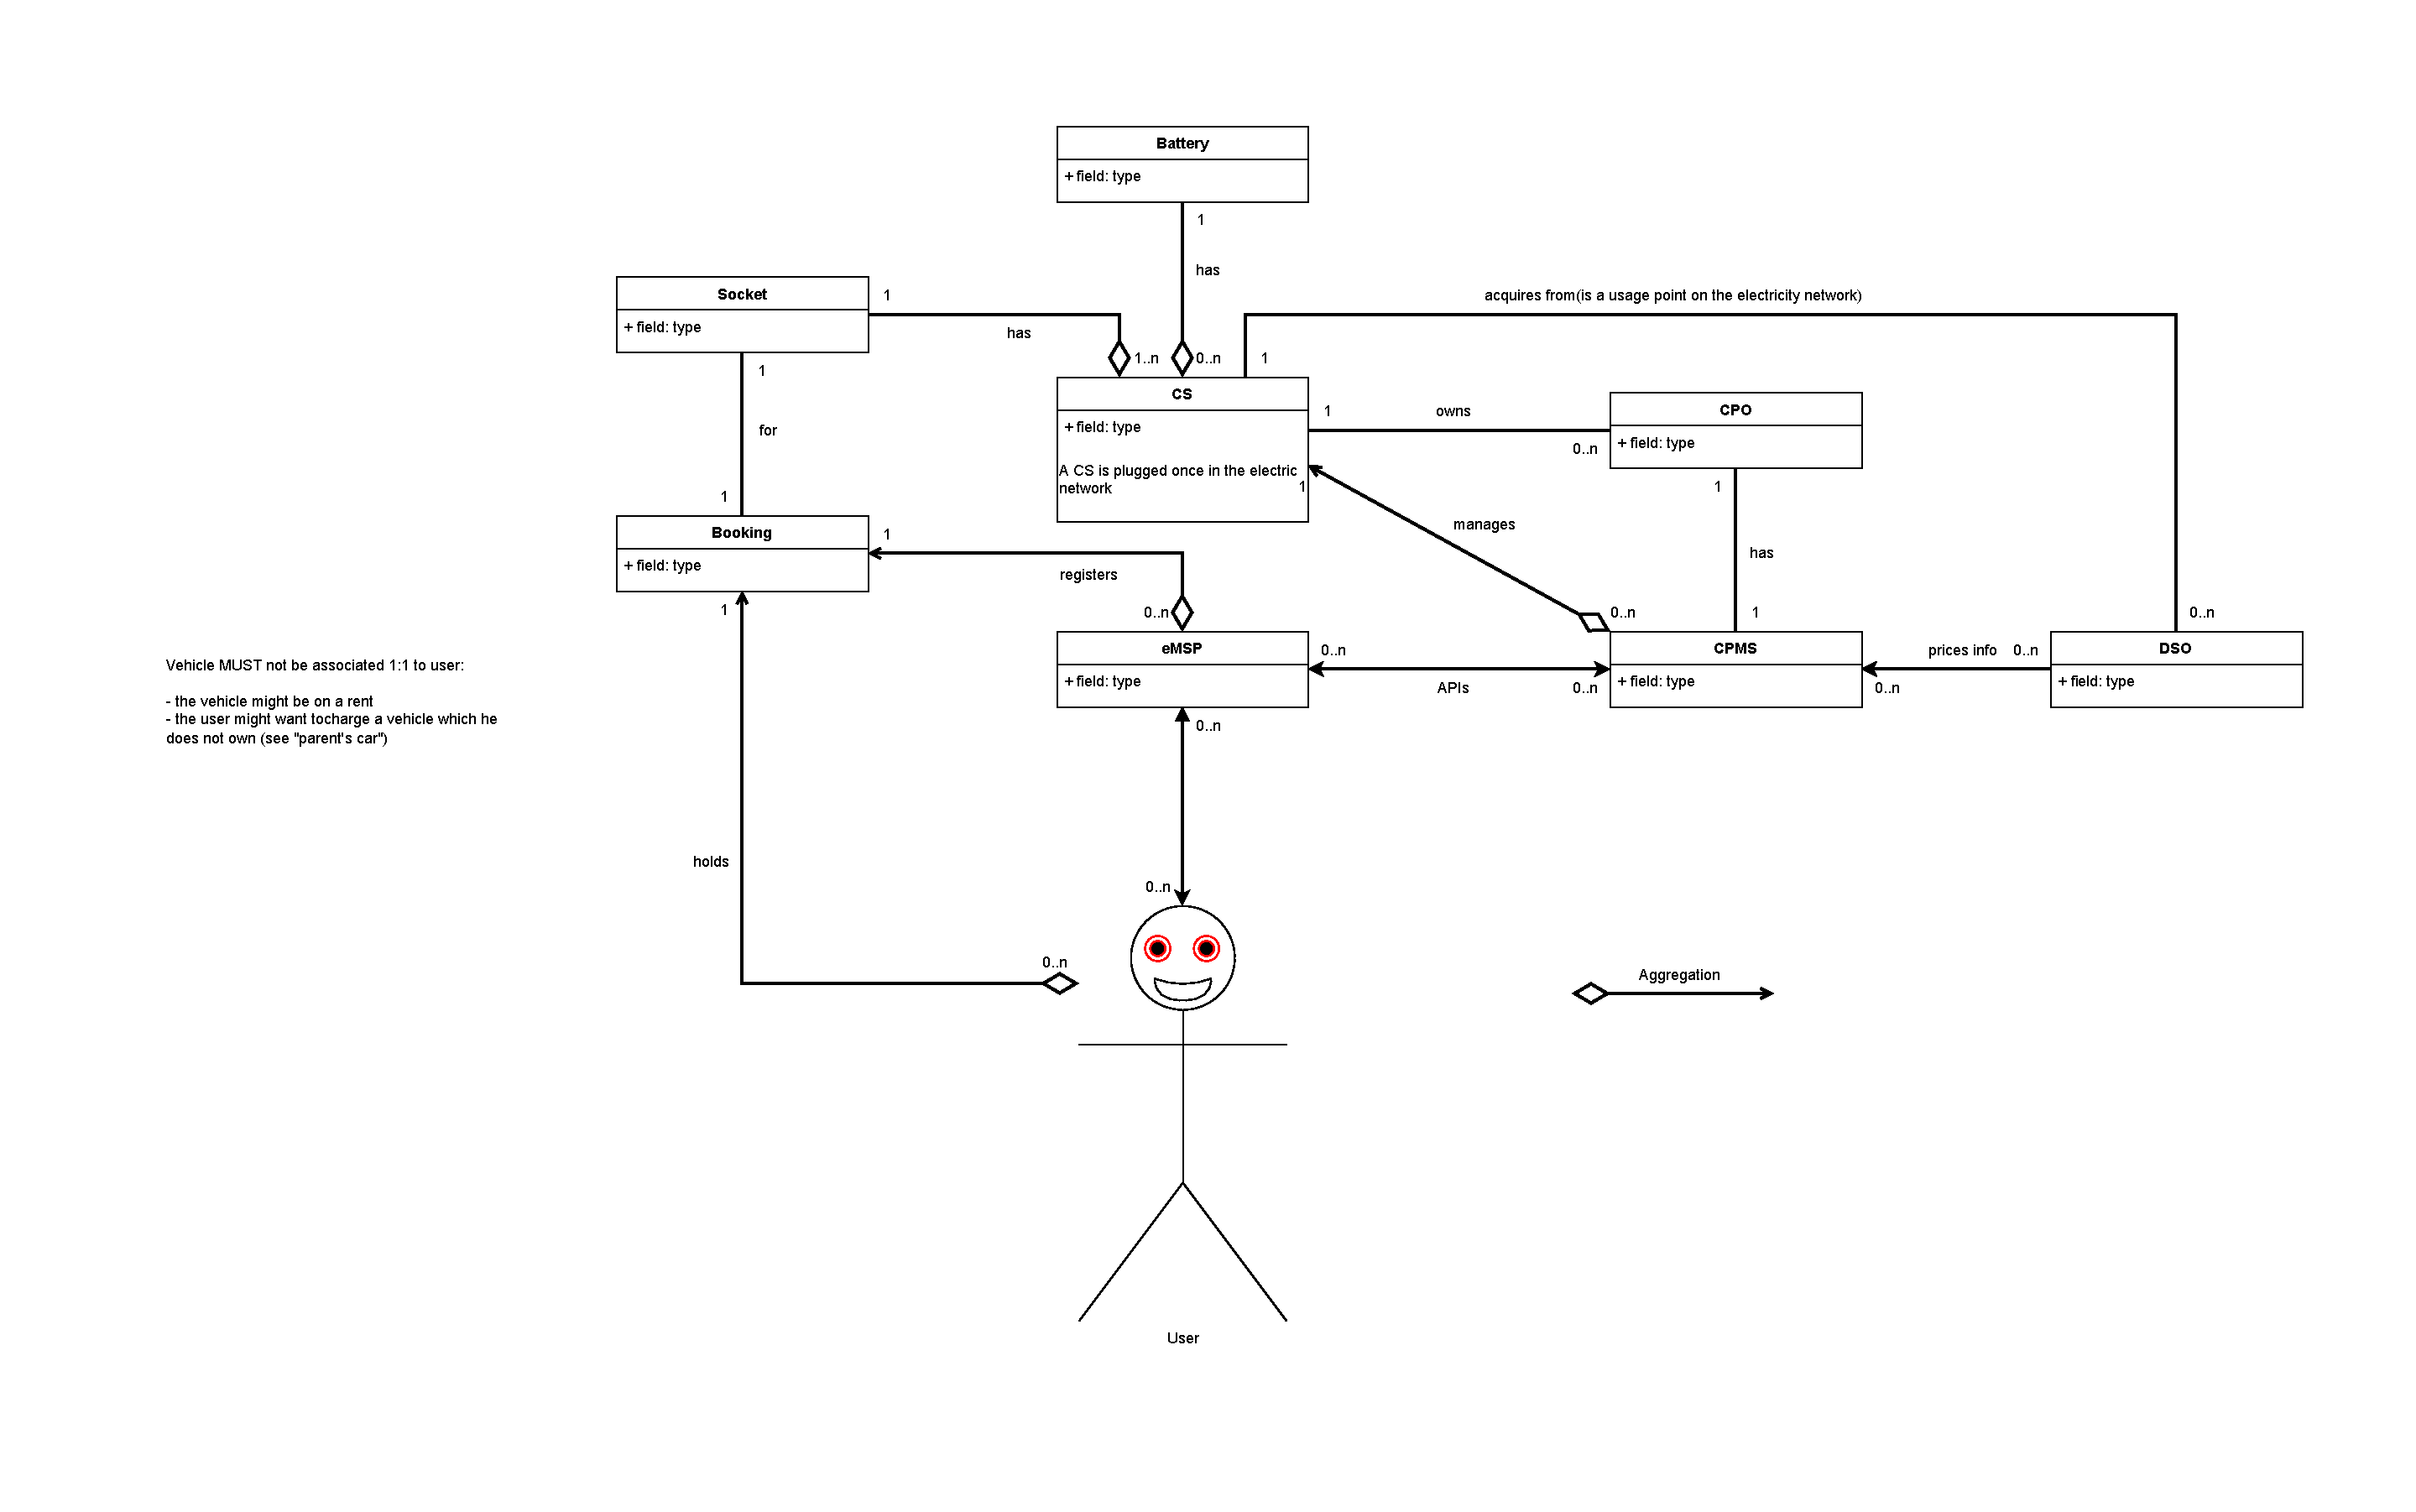
\includegraphics[page={1}, width=1.1\linewidth, trim=7.24cm 9cm 2.28cm 0cm, clip]{UML.pdf} %angle=-90
    }
    \caption{Class diagram}
\end{figure}

\newpage

\subsubsection{State Diagrams}

Those following are representations of the most important interactions that involve the STB, they mostly correspond to the different \hyperref[subsubsec:scenarios]{scenarios}.

\begin{description}
    \item \textbf{1. User registration and/or login}
    \begin{figure}[!ht]
        %trim = left bottom right top
        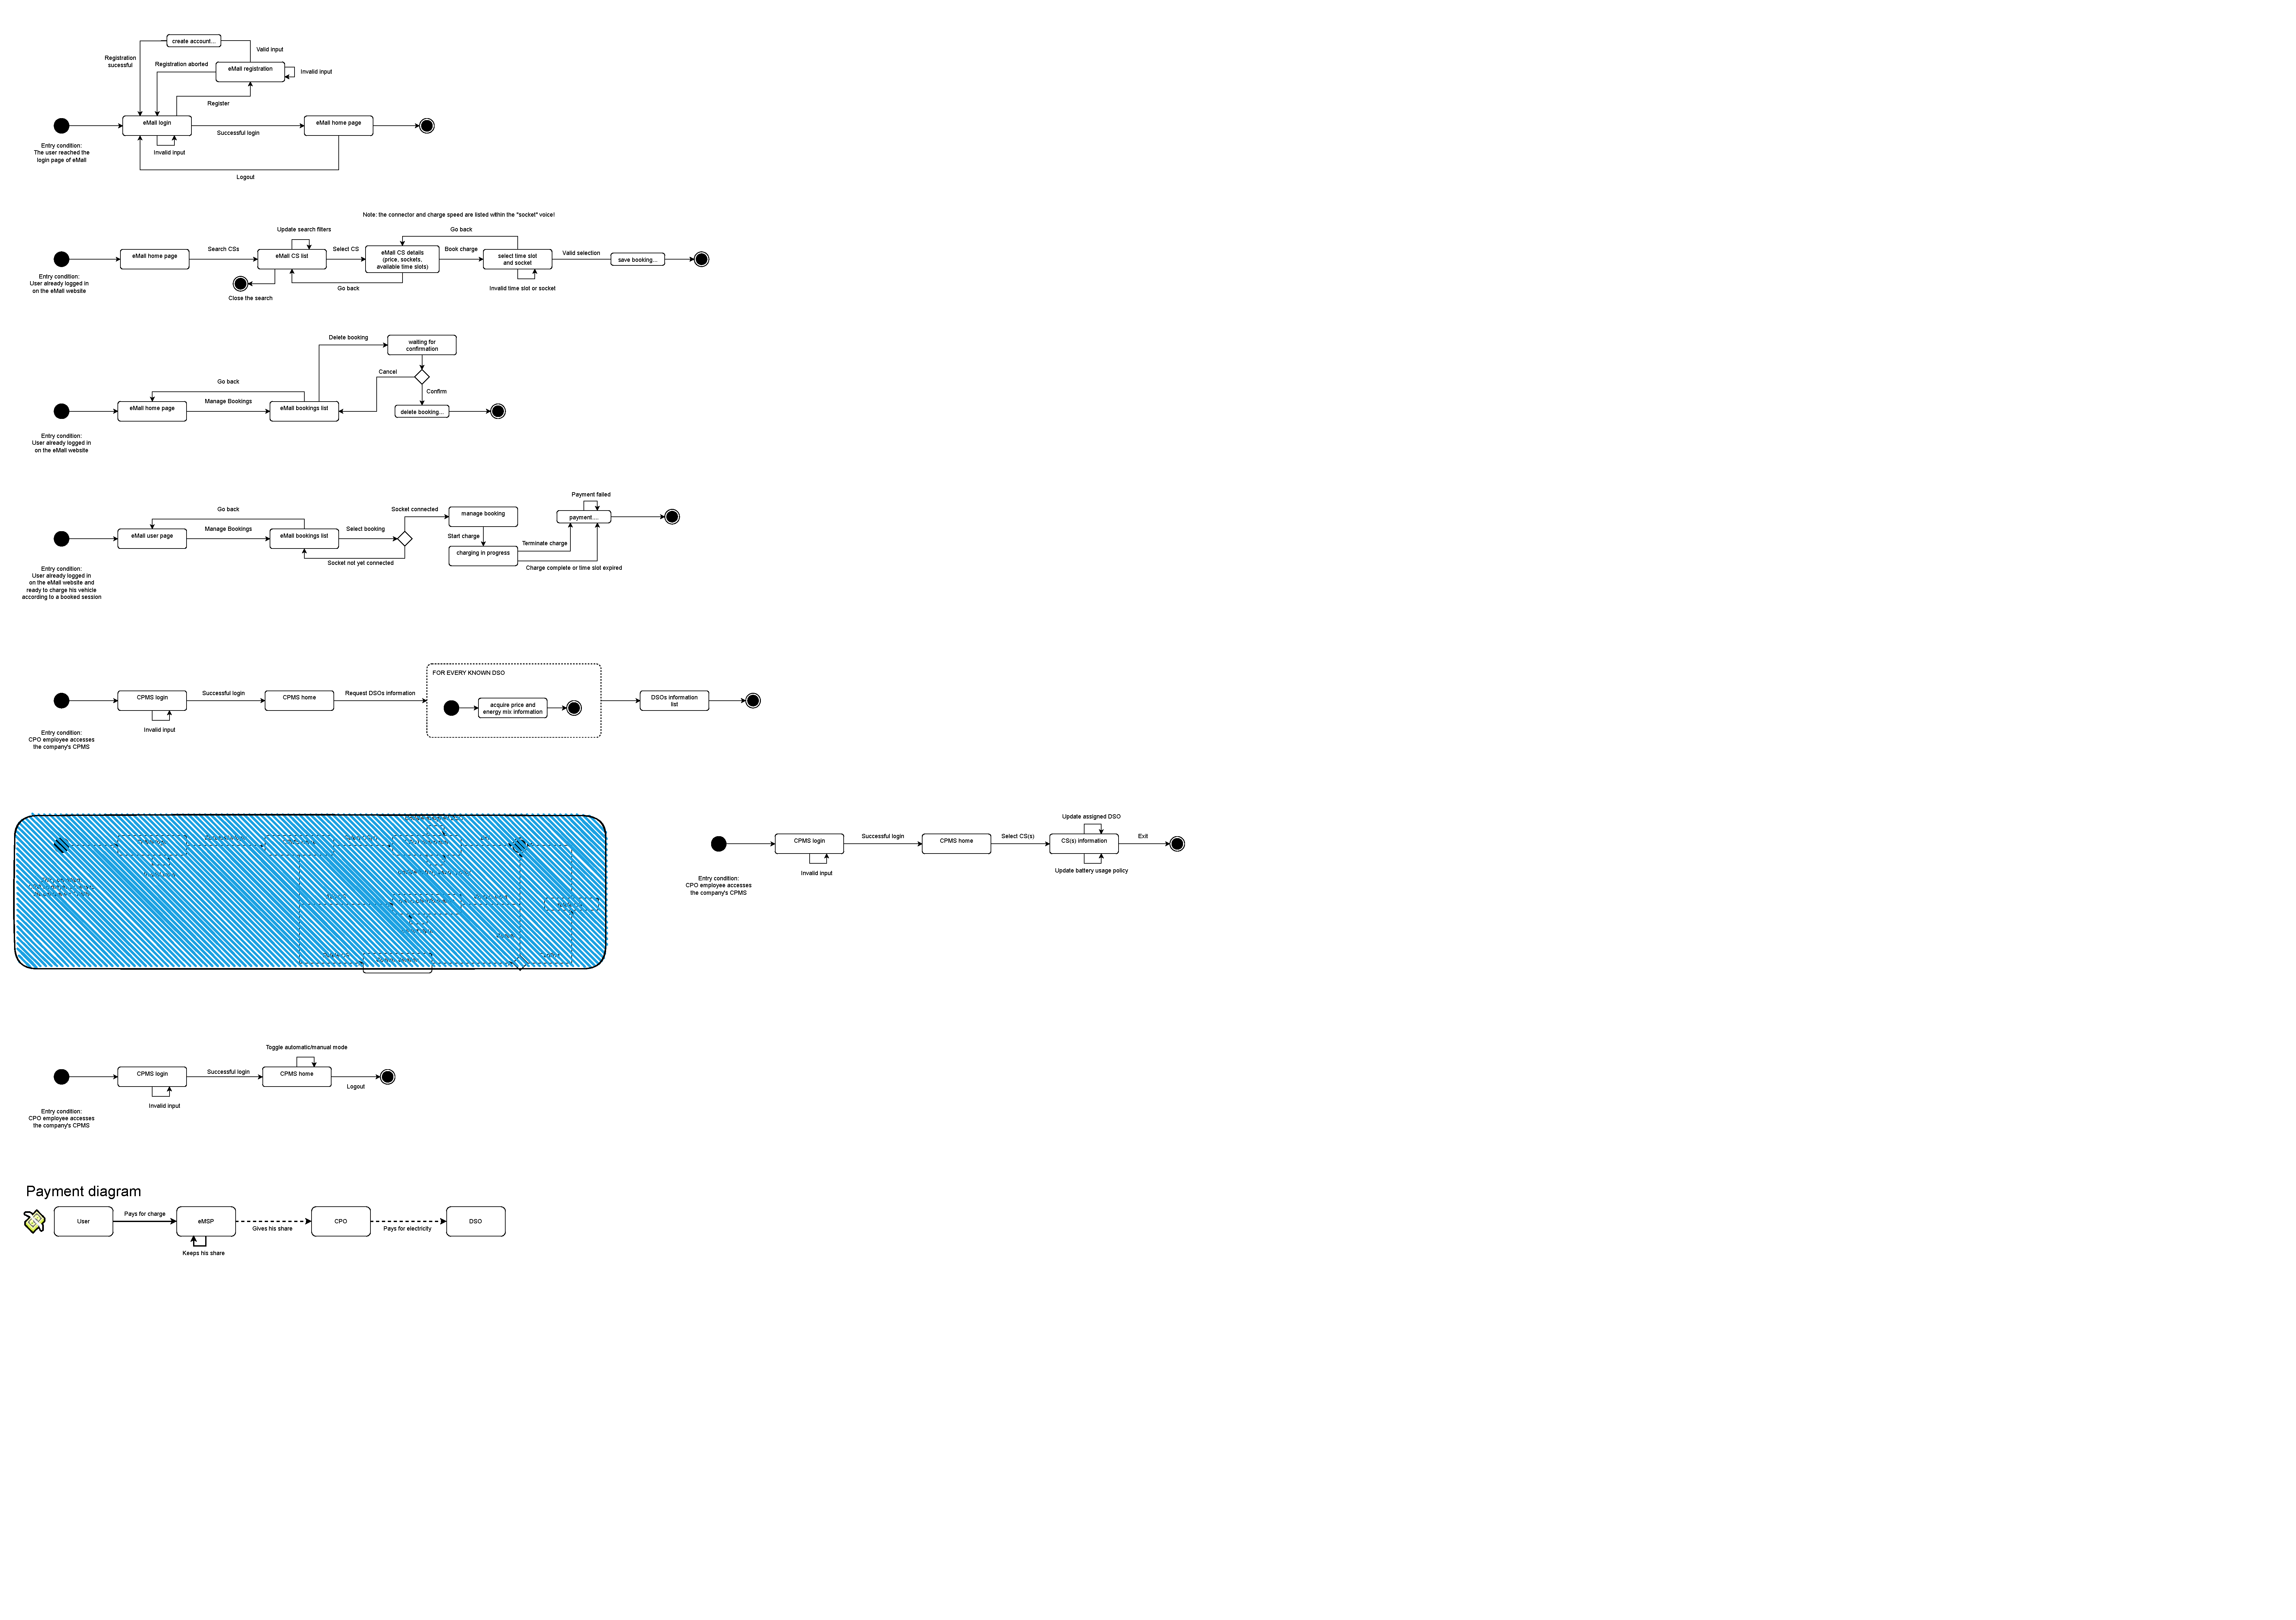
\includegraphics[page={1}, width=\linewidth, trim=8cm 3cm 8cm 3cm, clip]{StateCharts.pdf}
        \caption{User registration and/or login}
    \end{figure}
    
    \item \textbf{2. User searching CS and booking a recharge}
    \begin{figure}[!ht]
        %trim = left bottom right top
        \includegraphics[page={2}, width=\linewidth, trim=2cm 4cm 2cm 4cm, clip]{StateCharts.pdf}
        \caption{User searching CS and booking a recharge}
    \end{figure}
    
    \item \textbf{3. User deleting a booking}
    \begin{figure}[!ht]
        %trim = left bottom right top
        \includegraphics[page={3}, width=\linewidth, trim=7cm 4cm 7cm 4cm, clip]{StateCharts.pdf}
        \caption{User deleting a booking}
    \end{figure}
    
    \newpage
    
    \item \textbf{4. User performing a charging session}
    \begin{figure}[!ht]
        %trim = left bottom right top
        \includegraphics[page={4}, width=\linewidth, trim=2cm 4cm 2cm 4cm, clip]{StateCharts.pdf}
        \caption{User performing a charging session}
    \end{figure}
    
    \item \textbf{5. CPO acquiring information on DSOs' energy prices and mixes}
    \begin{figure}[!ht]
        %trim = left bottom right top
        \includegraphics[page={5}, width=\linewidth, trim=1cm 4cm 1cm 4cm, clip]{StateCharts.pdf}
        \caption{CPO acquiring information on DSOs' energy prices and mixes}
    \end{figure}
    
    \item \textbf{6. CPO chooses energy sources and battery usage policies for a CS}
    \begin{figure}[!ht]
        %trim = left bottom right top
        \includegraphics[page={6}, width=\linewidth, trim=6cm 5cm 6cm 5cm, clip]{StateCharts.pdf}
        \caption{CPO chooses energy sources and battery usage policies for a CS}
    \end{figure}
    
    \item \textbf{7. CPO toggles the CPMS automatic mode}
    \begin{figure}[!ht]
        %trim = left bottom right top
        \includegraphics[page={7}, width=\linewidth, trim=10cm 5cm 10cm 5cm, clip]{StateCharts.pdf}
        \caption{CPO toggles the CPMS automatic mode}
    \end{figure}
\end{description}

\subsection{Product Functions}
\label{subsec:prodfunctions}

\subsubsection{User registration}

eMall will allow Users to register an account. A User will register by entering:
\begin{itemize}
    \item A desired UserName
    \item Their email address
    \item A password
    \item A payment method
\end{itemize}
Given those data the account will be created and will be available to the User. This functionality will allow only one account to be bound to a specific email address.

\subsubsection{Search for CSs}
\label{subsubsection:searchForCS}

Users with an account will be able to search for CSs, multiple selectors will be available to narrow or widen the scope of the search, hence allowing Users to find the best result for their needs. Available filters will be:
\begin{itemize}
    \item Geographical area of interest
    \item Reharge price ranges
    \item Connector types available
    \item Charging speeds available
\end{itemize}
Users will be able to select a specific CS, consequently seeing the already booked time slots for it and further details as:
\begin{itemize}
    \item Location
    \item Price
    \item Offers
    \item Booking schedule
    \item Available connectors
    \item Available charging speeds
\end{itemize}

\subsubsection{Book a recharge at a CS}

From the list of results for the \hyperref[subsubsection:searchForCS]{\textbf{search for a CS}} a User will be able to book a recharge at a CS, they will be able to select a specific socket and time slot among the available ones for the CS and reserve it for themselves. During their booked time slot they will then have to show up at the CS with their vehicle to perform the recharge.

\subsubsection{Perform a recharge at a CS}

When the User show up at a CS during the time slot the booked it for and they connect to the booked socket they will be able to log into eMall, reach their bookings and start the charging process for the one they are currently connected for. Once the charging process is going, the User will be able to interrupt it through eMall at any time, otherwise the recharge will terminate after the vehicle is fully charged or the time slot expires, notifying the User. After the completion of a recharge the User will be charged by eMall for the service.

\subsection{Acquire price and energy mix information from DSOs}

A CPO will be able to ask their CPMS to present them with the information regarding energy prices and mix of energy sources used by the different DSOs known to the system. The CPMS will recover the information from DSOs and return it to the CPO.

\subsubsection{Choose prices, energy sources and battery usage policies for a CS}

The CPMS will provide its CPO with a list of all CSs handled by the system, from that list the CPO will be able to modify the configuration of each CS independently, specifically they will be able to alter the nominal-price and user-price, the DSO that is currently supplying that CS and the policy with which that CS used its batteries.

\subsubsection{Allow the CPMS to operate automatically}

The CPO will as well be able to let the CPMS take decisions regarding the prices, DSO and energy source of a CS automatically on their behalf.

\subsection{User Characteristics}

\begin{description}
    \item [1. Unregistered User] \hfill \\
        A User which just accesses the list of available CS without being able to book recharges, he has the option to register and become a \textit{Logged-In User} at any time.
    \item [2. Registered User] \hfill \\
        A User with a registered account within eMall which has yet to login-in with their credentials.
    \item [2. Logged-In User] \hfill \\
        A User with a registered account within eMall which has logged in via their credentials, can still access the CSs list and can also book a recharge. With their bookings he can then manage their charging sessions one he arrives at the CS.
    \item [3. CPO] \hfill \\
        By CPO at large we mean a company whose employees have access to the company's CPMS, hence the actual human beings interacting with the STB will be CPO employees with credentials that allow them to authenticate with the CPMS. The tasks an employee might perform are acquiring DSOs' information, assigning a DSO to a CS owned by their company, changing the battery management policy for any CS controlled by the CPMS or adding/updating CS managed by the CPMS. \\
        The reason for CPOs being identified as a users instead of their employees is that the decisions justifying the operations performed by the employees cannot be taken by the employees, they are just the executors, decisions are taken by their superiors, hence we can view of the entire company as a user to avoid being too specific about who takes which decision and who interacts with the STB. \\
        Furthermore a CPO is likely to use its information system to interface with the CPMS, hence identifying the company as a user also prevents distintions between direct CPMS access or access via the information system.
\end{description}

\subsection{Assumptions, Dependencies and Constraints}

\subsubsection{Domain Assumption}

\begin{table}[H]
    \centering
    %space between text and right/left borders
    \setlength{\tabcolsep}{18pt}
    %Row height multiplier
    \renewcommand{\arraystretch}{1.2}
    \begin{tabularx}{\textwidth}{|>{\centering\hsize=0.3\hsize}X|>{\hsize=1.7\hsize}X|}
        \hline
        \textbf{Assumption} & \textbf{Description} \\
        \hline
        %D1 & To change the sockets of a CS, the whole CS needs to be replaced \\
        D1 & CSs never disconnect from their CPMSs nor malfunction in any way as long as they are booked or in use \\
        \hline
        D2 & The only way to charge at a CS is by booking it via the eMSP \\
        \hline
        D3 & CSs are aware of whether a vehicle is connected or not, and if it is connected they know its charging state \\
        \hline
        D4 & CSs have the information required to reach out to their CPMS and connect to it by themselves, placing themselves under its control \\
        \hline
        D5 & No vehicle is connected to a socket of a CS at any given time unless it's booked for that time slot \\
        \hline
        D6 & The only user using a socket of a CS during a given time slot is the one who booked said socket \\
        \hline
        D7 & No vehicle is ever disconnected from a socket unless no charging process is in progress \\
        \hline
        D8 & A DSO's energy price is constant for all the locations where said DSO serves electricity \\
        \hline
        D9 & A DSO's energy mix is constant for all the locations where said DSO serves electricity \\
        \hline
        %D8 & The DSO association can be controlled on a per-CS basis and there is enough information provided by the DSOs to the CPMS to allow the latter to set a price for a charge at a CS and keep it constant during the whole process, while preventing that a DSO's price change causes a loss \\
        D10 & The user-price for a recharge at a CS is kept constant during the whole charging process \\
        \hline
        D11 & CPOs pay DSOs for the used electricity via methods outside the scope of this document (Ex: direct bank transfer) \\
        \hline
    \end{tabularx}
    \label{tab:domain_assumptions}
\end{table}

\newpage

\section{Specific Requirements}
\label{section:specificRequirements}

\subsection{External Interface Requirements}

\subsubsection{User Interfaces}

The interface eMall will use is a web app, through which its Users will have available all \hyperref[subsec:prodfunctions]{product functions}. Such web app will need to be usable both on desktop and mobile devices, since a mobile device is what users will most likely have available to them while at the CS. \\
\\
MOCKUPS HERE \\
\\
Similarly, CPMSs will offer their functionality to CPOs via a web portal, here there is no need to support anything other than a desktop device, since CPMSs are intended to be managed by employees in a company environment.

\subsubsection{Hardware Interfaces}

Users will require a device equipped with a web browser and an internet connection to access the eMall website, the hardware architecture of the specific device is irrelevant as long as it runs an OS equipped with a web browser. \\
\\
CPOs will as well only require a device capable of web browsing, although in this case such device is intended to a be a desktop machine since its users will be the employees working at the CPOs from their offices. \\
\\
CSs will need to be equipped with adequate hardware to monitor each socket and control circuitry for their batteries, if there are any connected to them. Furthermore CSs need to connect to and communicate with their respective CPMSs, hence a small computer within each CS capable of collecting sockets and battery(ies) data as well as interface with the internet (via 4G or a wired connection) is necessary. \\
Furthermore this document will assume that a CS is billed for its used electricity via a in loco electricity meter independently monitored by the DSO currently assigned to the CS by the CPMS.

\subsubsection{Software Interfaces}
%The information exchanged between different SW entities in the same "location"

Devices in the end of eMSP users will require an OS equipped with a network stack within which to run a web browser. The same is true on the CPOs side, on their machines there need to be an OS with network capabilities suitable for a web browser. \\
\\
%A software dedicated to handling payments is required for the eMSP, in order to allow it to charge users when needed using the payment method details stored by the eMSP. Such software needs to be invokeable by the eMSP at any time. \\
%\\
The computer installed on CS will need to have an OS with networking capabilities too, while also having adequate software to collect and process the information coming from the CS's sockets and eventually connected vehicles, as well as to manage eventual batteries connected to the CS.

%Map service and payment system...

\subsubsection{Communication Interfaces}
%The medium over which information is exchanged

%ADD: interface for the CS that automatically connect to the CPMS on their own!

The main functionalities of the STB require cooperation of multiple components sometimes owned by different parties and not deployed on machines in the same local network, hence their interactions occur via adequate web APIs. The interactions requiring such interfaces are the following:

\begin{description}
    \item [1. eMSP acquiring CS information from CPMSs] \hfill \\
        Whenever a search for CSs, a booking or a recharge at a CS is performed via an eMSP, the ladder needs to fetch information regarding one or more CSs from CPMSs first, hence CPMSs need to expose a web API reachable by the eMSP to communicate the details regarding CSs.
    \item [2. eMSP  managing a recharge through a CPMS] \hfill \\
        When a charging process for a previous booking needs to be starter or terminated by a user via the eMSP, the eMSP has no control over the CS, hence needs to interface with the CPSM to request the latter to start/stop the charging process. Hence the CPMS needs to expose in it web API method for eMSP to start/stop charging procedures that were booked through them.
    \item [3. eMSP requesting a payment via an external provider] \hfill \\
        After the completion of a charging process or when a fee is charged to a user, the eMSP needs to use the payment method a user has bound to its account to charge them for the service, hence it needs to interface with an API which will allow the eMSP to have the amount due accredited to himself.
    \item [4. CPMS monitoring and controlling its CSs] \hfill \\
        CSs need to know how to reach the CPMS responsible for them over internet, this way whenever a CS is deployed it will automatically find its CPMS, authenticate with it and setup itself under its control. To this end CPMSs need to expose a web API allowing for new CSs to authenticate with them, and CSs need to offer the connect CPMS and endpoint to allow it to manage them.
    \item [5. CPMS acquiring DSOs price and energy mix information] \hfill \\
        To allow CPMSs to know their energy prices and mixes, DSO must have an API available via web so that CPMSs can recover such information.
\end{description}

\subsection{Functional Requirements}

\subsubsection{Requirement assertions}

\begin{table}[H]
    \centering
    %space between text and right/left borders
    \setlength{\tabcolsep}{18pt}
    %Row height multiplier
    \renewcommand{\arraystretch}{1.2}
    \begin{tabularx}{\textwidth}{|>{\centering\hsize=0.1\hsize}X|>{\hsize=1.9\hsize}X|}
        \hline
        \textbf{Id} & \textbf{Requirement} \\
        \hline
        R1 & The eMSP shall allow a registered user to login \\
        \hline
        R2 & The eMSP shall allow an unregistered user to register on the platform \\
        \hline
        %Maybe specialize for each error
        %Maybe errors -> invalid input
        R3 & The eMSP should report to the user when they sent invalid input data through a form \\
        \hline
        R4 & The eMSP should report to the user when they attempted to perform an unauthorized action \\
        \hline
        R5 & The eMSP should report to the user when the platform encountered an error while processing the action \\
        \hline
        R6 & The eMSP should report to the user any successful action performed \\
        \hline
        R7 & The eMSP shall allow a logged-in user to view charging stations nearby \\
        \hline
        R8 & The eMSP shall allow a logged-in user to know the cost of a recharge at a CS \\
        \hline
        R9 & The eMSP shall allow a logged-in user to know about ongoing special offers present at a CS \\
        \hline
        R10 & The eMSP shall allow a logged-in user to book a recharge at a free socket of a CS for a given time slot \\
        \hline
        R11 & The eMSP shall allow a logged-in user to cancel any of its booked recharges \\
        \hline
        R12 & The eMSP shall not allow a user to book a recharge at a socket of a CS which has already been booked for the chosen time slot \\
        \hline
        R13 & The eMSP shall not allow a user to book multiple recharges with overlapping time slots \\
        \hline
        R14 & The eMSP shall allow a logged-in user to start the charging process for one of their booked recharges \\
        \hline
    \end{tabularx}
    \label{tab:requirements}
\end{table}

\begin{table}[H]
    \centering
    %space between text and right/left borders
    \setlength{\tabcolsep}{18pt}
    %Row height multiplier
    \renewcommand{\arraystretch}{1.2}
    \begin{tabularx}{\textwidth}{|>{\centering\hsize=0.1\hsize}X|>{\hsize=1.9\hsize}X|}
        \hline
        \textbf{Id} & \textbf{Requirement} \\
        %IMPLIES ONLY A RECHARGE ONGOING AT ANY GIVEN TIME
        \hline
        R15 & The eMSP shall not allow a user without a booking to start the charging process \\
        \hline
        R16 & The eMSP shall not allow a user to start the charging process as long as the socket is vacant \\
        \hline
        R17 & The eMSP should notify a logged-in user when their ongoing charging processes is complete \\
        \hline
        R18 & The eMSP should notify a logged-in user when their ongoing charging process is terminated due to the expiration of its booked time slot \\
        \hline
        R19 & The eMSP shall allow a logged-in user to terminate their charging process earlier \\
        \hline
        R20 & The eMSP should charge a user for everyone of his charging processes as soon as they finish \\
        \hline
        R21 & The eMSP shall charge a user for a fee if they do not start a recharge during their booking's time slot \\
        \hline
        R22 & The eMSP shall be able to offer its functionalities to multiple users at once \\
        \hline
        R23 & The eMSP shall be able to pay CPOs for the amount due for recharges performed through them since the last payment \\
        \hline
        R24 & The CPMS should be able to acquire location from CSs \\
        \hline
        R25 & The CPMS should be able to acquire the internal status from CSs \\
        \hline
        R26 & The CPMS should be able to acquire the external status from CSs \\
        \hline
        R27 & The CPMS should be able to start charging a vehicle connected to a CS socket \\
        \hline
        R28 & The CPMS should be able to monitor the charging process of a vehicle \\
        \hline
        R29 & The CPMS should be able to acquire from DSOs their current energy prices \\
        \hline
        R30 & The CPMS should be able to acquire from DSOs their energy mix \\
        \hline
        R31 & The CPMS shall allow its CPO to assign a DSO to a CS as its energy provider  when operating in “Manual Mode” \\
        \hline
        R32 & The CPMS should be able to automatically assign a DSO to a CS as its energy provider when operating in “Automatic Mode” \\
        \hline
        %the policy is ONE for the whole CPMS and the CURRENT energy source is one PER-CS!
        R33 & The CPMS shall allow the CPO to decide the energy source management policies when operating in “Manual Mode” \\
        \hline
        R34 & The CPMS should be able to automatically choose the current energy source for a CS according to the given policy when operating in “Automatic Mode” \\
        \hline
        R35 & The CPMS shall allow its CPO to assign a nominal-price and a user-price to a CS when operating in “Manual Mode” \\
        \hline
        R36 & The CPMS should be able to automatically assign a nominal-price and a user-price to a CS when operating in “Automatic Mode” \\
        \hline
        R37 & The CPMS shall allow the CPO to choose its policies for operating in "Automatic Mode" \\
        \hline
        R38 & The CPMS shall allow the CPO to choose whether it acts automatically or manually \\
        \hline
        R39 & The CPMS shall never take a decision automatically when it is set in “Manual Mode” \\
        \hline
        R40 & The CPMS should report to the user when they sent invalid input data \\
        \hline
        R41 & The CPMS should report to the user when they attempted to perform an unauthorized action \\
        \hline
        \end{tabularx}
    \label{tab:requirements}
\end{table}

\begin{table}[H]
    \centering
    %space between text and right/left borders
    \setlength{\tabcolsep}{18pt}
    %Row height multiplier
    \renewcommand{\arraystretch}{1.2}
    \begin{tabularx}{\textwidth}{|>{\centering\hsize=0.1\hsize}X|>{\hsize=1.9\hsize}X|}
        \hline
        \textbf{Id} & \textbf{Requirement} \\
        \hline
        R42 & The CPMS should report to the user when the platform encountered an error while processing the action \\
        \hline
        % AUTOMATIC PAYMENT TO DSOs?????????
        %R43 & The CPMS should be able to pay DSOs the amount due for the recharges performed with its energy \\
        %\hline
        %R41 & The CPMS should be able to set special offers on CSs for a set time interval \\
        %\hline
        R43 & The CPMS should be able to decide whether to start charging the internal batteries of a CS (if present) \\
        \hline
    \end{tabularx}
    \label{tab:requirements-2}
\end{table}

\subsubsection{Mapping on goals}

\begin{table}[H]
    \centering
    %space between text and right/left borders
    \setlength{\tabcolsep}{18pt}
    %Row height multiplier
    \renewcommand{\arraystretch}{1.2}
    \begin{tabularx}{\textwidth}{|>{\hsize=0.4\hsize}X|>{\hsize=1\hsize}X|>{\hsize=1.6\hsize}X|}
        \hline
        \textbf{Goal} & \textbf{Domain assumption} & \textbf{Requirement} \\
        \hline
        G1 & D4 & R1, R2, R3, R4, R5, R6, R7, R22, R24, R26 \\ %List
        \hline
        G2 & D4, D8, D9 & R1, R2, R3, R4, R5, R6, R8, R9, R22, R26, R29, R30 \\ %Cost
        \hline
        G3 & D1, D2, D4 & R1, R2, R3, R4, R5, R6, R7, R10, R11, R12, R13, R21, R22, R24, R26 \\ %Book
        \hline
        G4 & D1, D2, D3, D4, D5, D6, D7, D10, D11 & R1, R2, R3, R4, R5, R6, R14, R15, R16, R17, R18, R19, R20, R23, R25, R26, R27, R28, R29 \\ %Monitor
        \hline
        G5 & D8, D9, D11 & R29, R30, R31, R32, R33, R34, R35, R36, R37, R38, R39, R40, R41, R42, R43 \\ %Energy Source
        \hline
    \end{tabularx}
    \label{tab:requirementsMapping}
\end{table}

\newpage

\subsubsection{Use cases}
%MAYBE BEFORE REQUIREMENTS

\begin{description}
    \item [1. New user registration] \hfill \\
    \begin{table}[H]
        \centering
        %space between text and right/left borders
        \setlength{\tabcolsep}{18pt}
        %Row height multiplier
        \renewcommand{\arraystretch}{1.4}
        \begin{tabularx}{\textwidth}{|>{\hsize=0.5\hsize}X|>{\hsize=1.5\hsize}X|}
            \hline
            \textbf{Actor} & Unregistered User \\
            \hline
            \textbf{Entry condition} & The User does not have an eMall account yet and reached eMall's login page \\
            \hline
            \textbf{Event flow} & 
                \begin{minipage}[t]{\hsize}
                \begin{enumerate}[topsep=0pt, leftmargin=*]
                    \item The User selects the option to register on eMall
                    \item The User enters his desired UserName for the platform, his email address, a password and a payment method for his new account
                    \item The User submits the inserted data to eMall
                    \item eMall registers the account and the User can now log in with it
                \end{enumerate}
                \end{minipage}
                \vspace{6pt}
            \\
            \hline
            \textbf{Exit condition} & The User's account has been created \\
            \hline
            \textbf{Exceptions} & 
                \begin{minipage}[t]{\hsize}
                \vspace{0pt}
                \begin{itemize}[topsep=0pt, leftmargin=*]
                    \item The User's inserted data was not complete or did not comply with the requested formats
                    \item The User's email is already associated to an existing account
                \end{itemize}
                \vspace{8pt}
                \end{minipage}
                In all those situation an error is presented to the User.
                \vspace{6pt}
            \\
            \hline
        \end{tabularx}
    \end{table}
    
    \item [2. User login] \hfill \\
    \begin{table}[H]
        \centering
        %space between text and right/left borders
        \setlength{\tabcolsep}{18pt}
        %Row height multiplier
        \renewcommand{\arraystretch}{1.4}
        \begin{tabularx}{\textwidth}{|>{\hsize=0.5\hsize}X|>{\hsize=1.5\hsize}X|}
            \hline
            \textbf{Actor} & Registered User \\
            \hline
            \textbf{Entry condition} & The User already has an eMall account, is not currently logged-in, and reached eMall's login page \\
            \hline
            \textbf{Event flow} & 
                \begin{minipage}[t]{\hsize}
                \begin{enumerate}[topsep=0pt, leftmargin=*]
                    \item The User selects the option to log in on eMall
                    \item The User enters his account's email and password
                    \item The User submits the inserted data to eMall
                    \item eMall verifies the credential's validity and presents the user with the home page
                \end{enumerate}
                \end{minipage}
                \vspace{6pt}
            \\
            \hline
            \textbf{Exit condition} & The User logged in on eMall \\
            \hline
            \textbf{Exceptions} & 
                \begin{minipage}[t]{\hsize}
                \vspace{0pt}
                \begin{itemize}[topsep=0pt, leftmargin=*]
                    \item The User's inserted data was not complete or did not comply with the requested formats
                    \item The User's credentials were not valid for any account
                \end{itemize}
                \vspace{8pt}
                \end{minipage}
                In all those situation an error is presented to the User.
                \vspace{6pt}
            \\
            \hline
        \end{tabularx}
    \end{table}
    
    \newpage
    
    \item [3. User searching and booking a CS] \hfill \\
    \begin{table}[H]
        \centering
        %space between text and right/left borders
        \setlength{\tabcolsep}{18pt}
        %Row height multiplier
        \renewcommand{\arraystretch}{1.4}
        \begin{tabularx}{\textwidth}{|>{\hsize=0.5\hsize}X|>{\hsize=1.5\hsize}X|}
            \hline
            \textbf{Actor} & Logged-in User \\
            \hline
            \textbf{Entry condition} & The User has already logged in and is on eMall's home page \\
            \hline
            \textbf{Event flow} & 
                \begin{minipage}[t]{\hsize}
                \begin{enumerate}[topsep=0pt, leftmargin=*]
                    \item The User selects the “search” option for CSs  
                    \item The User is presented with an initial list of CSs (could be empty) and the filters to update the search results \hyperref[scenario:lookingForCS]{\textbf{(filters list here)}}
                    \item The User can repeat the search to his hearth's contempt by updating the filters
                    \item The User selects a CS to be shown its details \hyperref[scenario:lookingForCS]{\textbf{(details list here)}}
                    \item The User chooses to book a recharge at the selected CS
                    \item The User inserts the desired socket and time slot for his booking
                    \item eMall registers the User's booking and confirms it to the User
                \end{enumerate}
                \end{minipage}
                \vspace{6pt}
            \\
            \hline
            \textbf{Exit condition} & The User booked a recharge at a CS \\
            \hline
            \textbf{Exceptions} & 
                \begin{minipage}[t]{\hsize}
                \vspace{0pt}
                \begin{itemize}[topsep=0pt, leftmargin=*]
                    \item The User's inserted values in filters did not comply with accepted formats
                    \item The User's inserted data was not complete or did not comply with the requested formats
                    %IMPORTANT: NO TWO BOOKINGS ON THE SAME CS's SOCKET SHOULD EVER OVERLAP
                    \item The User's selected socket is already occupied for the chosen time slot
                    %IMPORTANT: NO TWO BOOKINGS OF THE SAME USER SHOULD EVER OVERLAP
                    \item The User already has another booking that presents an overlapping time slot with the currently selected one
                \end{itemize}
                \vspace{8pt}
                \end{minipage}
                In all those situation an error is presented to the User.
                \vspace{6pt}
            \\
            \hline
        \end{tabularx}
    \end{table}
    
    \item [4. User deleting one of his bookings] \hfill \\
    \begin{table}[H]
        \centering
        %space between text and right/left borders
        \setlength{\tabcolsep}{18pt}
        %Row height multiplier
        \renewcommand{\arraystretch}{1.4}
        \begin{tabularx}{\textwidth}{|>{\hsize=0.5\hsize}X|>{\hsize=1.5\hsize}X|}
            \hline
            \textbf{Actor} & Logged-in User \\
            \hline
            \textbf{Entry condition} & The User has already logged in and is on eMall's home page \\
            \hline
            \textbf{Event flow} & 
                \begin{minipage}[t]{\hsize}
                \begin{enumerate}[topsep=0pt, leftmargin=*]
                    \item The User selects the option to see his bookings' list
                    \item The User selects the booking they want to delete from the list
                    \item The User chooses the delete option on the selected meeting
                    \item eMall deletes the selected booking and confirms it to the User
                \end{enumerate}
                \end{minipage}
                \vspace{6pt}
            \\
            \hline
            \textbf{Exit condition} & The User logged in on eMall \\
            \hline
            %SHALL WE INCLUDE "MEETING NOT FOUND"? Or that's too implementation stuff...
            \textbf{Exceptions} & No exception can happen during within user case. \\
            \hline
        \end{tabularx}
    \end{table}
    
    \newpage
    
    \item [5. User starting a charging process] \hfill \\
    \begin{table}[H]
        \centering
        %space between text and right/left borders
        \setlength{\tabcolsep}{18pt}
        %Row height multiplier
        \renewcommand{\arraystretch}{1.4}
        \begin{tabularx}{\textwidth}{|>{\hsize=0.5\hsize}X|>{\hsize=1.5\hsize}X|}
            \hline
            \textbf{Actor} & Logged-in User \\
            \hline
            \textbf{Entry condition} & The User has already logged in and is on eMall's home page, has arrived at a CS during their booked time slot and has connected their vehicle to the booked socket \\
            \hline
            \textbf{Event flow} & 
                \begin{minipage}[t]{\hsize}
                \begin{enumerate}[topsep=0pt, leftmargin=*]
                    \item The User selects the option to see his bookings' list
                    \item The User selects the booking made for the current time slot (eMall might highlight it ahead of time)
                    \item The User is presented with the booking's status and the option to start the charging process
                    \item The User chooses to start the charging process
                    \item eMall, via the CPMS, makes the CS's socket start to recharge the connected vehicle
                \end{enumerate}
                \end{minipage}
                \vspace{6pt}
            \\
            \hline
            \textbf{Exit condition} & The CS's socket started charging the connected vehicle \\
            \hline
            \textbf{Exceptions} & No exception can happen during within user case. \\
            \hline
        \end{tabularx}
    \end{table}
    
    \item [6. User interrupting a charging process] \hfill \\
    \begin{table}[H]
        \centering
        %space between text and right/left borders
        \setlength{\tabcolsep}{18pt}
        %Row height multiplier
        \renewcommand{\arraystretch}{1.4}
        \begin{tabularx}{\textwidth}{|>{\hsize=0.5\hsize}X|>{\hsize=1.5\hsize}X|}
            \hline
            \textbf{Actor} & Logged-in User \\
            \hline
            \textbf{Entry condition} & The User has already logged in and is on eMall's home page while his current booking has an ongoing charging process \\
            \hline
            \textbf{Event flow} & 
                \begin{minipage}[t]{\hsize}
                \begin{enumerate}[topsep=0pt, leftmargin=*]
                    \item The User selects the option to see his bookings' list
                    \item The User selects the booking made for the current time slot with the active charging process
                    \item The User is presented with the charging process's status and the option to interrupt it
                    \item The User chooses to interrupt the charging process
                    \item eMall, via the CPMS, makes the CS's socket stop the charging of the connected vehicle
                    \item eMall charges the User for the received service through adequate external services, using the User’s registered payment method
                \end{enumerate}
                \end{minipage}
                \vspace{6pt}
            \\
            \hline
            \textbf{Exit condition} & The booking's charging procedure has ended and the payment has succeeded \\
            \hline
            \textbf{Exceptions} & 
                \begin{minipage}[t]{\hsize}
                \vspace{0pt}
                \begin{itemize}[topsep=0pt, leftmargin=*]
                    \item The payment is rejected
                \end{itemize}
                \vspace{8pt}
                \end{minipage}
                In the above situation eMall retries the payment a given number of times, if it never succeeds eMall notifies the User to change their payment method.
                \vspace{6pt}
            \\
            \hline
        \end{tabularx}
    \end{table}
    
    \newpage
    
    \item [7. Charging procedure self-terminates and User receives a notification] \hfill \\
    \begin{table}[H]
        \centering
        %space between text and right/left borders
        \setlength{\tabcolsep}{18pt}
        %Row height multiplier
        \renewcommand{\arraystretch}{1.4}
        \begin{tabularx}{\textwidth}{|>{\hsize=0.5\hsize}X|>{\hsize=1.5\hsize}X|}
            \hline
            \textbf{Actor} & Logged-in User \\
            \hline
            \textbf{Entry condition} & The User has already logged in and is on eMall's home page while his current booking has just reached one of its termination conditions:
            \begin{minipage}[t]{\hsize}
            \begin{itemize}
                \item The booked time slot has expired
                \item The connected vehicle is completely charged
            \end{itemize}
            \end{minipage}
            \vspace{6pt}
            \\
            \hline
            \textbf{Event flow} & 
                \begin{minipage}[t]{\hsize}
                \begin{enumerate}[topsep=0pt, leftmargin=*]
                    \item eMall, via the CPMS, makes the CS's socket stop the charging of the connected vehicle if it hasn't already halted by itself
                    \item eMall charges the User for the received service through adequate external services, using the User’s registered payment method
                    \item The User receives a notification from eMall telling them that their charging procedure just ended
                \end{enumerate}
                \end{minipage}
                \vspace{6pt}
            \\
            \hline
            \textbf{Exit condition} & The booking's charging procedure has ended, the payment has succeeded and the User has been notified \\
            \hline
            \textbf{Exceptions} & 
                \begin{minipage}[t]{\hsize}
                \vspace{0pt}
                \begin{itemize}[topsep=0pt, leftmargin=*]
                    \item The payment is rejected
                        \vspace{6pt} \\
                        In this situation eMall retries the payment a given number of times, if it never succeeds eMall notifies the User to change their payment method.
                \end{itemize}
                \vspace{8pt}
                \end{minipage}
                \vspace{6pt}
                \begin{minipage}[t]{\hsize}
                \vspace{0pt}
                \begin{itemize}[topsep=0pt, leftmargin=*]
                    \item The User did not receive the notification
                    \vspace{6pt} \\
                    In this situation eMall send the notification again every predetermined amount of time for a configured number of attempts.
                \end{itemize}
                \vspace{8pt}
                \end{minipage}
            \\
            \hline
        \end{tabularx}
    \end{table}
    
    \item [8. User does not show up for a booked recharge] \hfill \\
    \begin{table}[H]
        \centering
        %space between text and right/left borders
        \setlength{\tabcolsep}{18pt}
        %Row height multiplier
        \renewcommand{\arraystretch}{1.4}
        \begin{tabularx}{\textwidth}{|>{\hsize=0.5\hsize}X|>{\hsize=1.5\hsize}X|}
            \hline
            \textbf{Actor} & Registered User \\
            \hline
            \textbf{Entry condition} & The Registered User had a booking with eMall whose time slot just expired without the User ever starting the charging process \\
            \hline
            \textbf{Event flow} & 
                \begin{minipage}[t]{\hsize}
                \begin{enumerate}[topsep=0pt, leftmargin=*]
                    \item eMall detects the the expiration of the breached booking
                    \item eMall charges the User a fee for the reservation
                \end{enumerate}
                \end{minipage}
                \vspace{6pt}
            \\
            \hline
            \textbf{Exit condition} & The payment of the fee succeeds \\
            \hline
            \textbf{Exceptions} & 
                \begin{minipage}[t]{\hsize}
                \vspace{0pt}
                \begin{itemize}[topsep=0pt, leftmargin=*]
                    \item The payment is rejected
                \end{itemize}
                \vspace{8pt}
                \end{minipage}
                In the above situation eMall retries the payment a given number of times, if it never succeeds eMall notifies the User to change their payment method.
                \vspace{6pt}
            \\
            \hline
        \end{tabularx}
    \end{table}
    
    \item [9. CPO requests information on DSOs’ energy prices and mix of sources] \hfill \\
    \begin{table}[H]
        \centering
        %space between text and right/left borders
        \setlength{\tabcolsep}{18pt}
        %Row height multiplier
        \renewcommand{\arraystretch}{1.4}
        \begin{tabularx}{\textwidth}{|>{\hsize=0.5\hsize}X|>{\hsize=1.5\hsize}X|}
            \hline
            \textbf{Actor} & CPO (employee) \\
            \hline
            \textbf{Entry condition} & A CPO employee has authorized access to the company's CPMS and performing this task is part of his job, hence reached the CPMS login page \\
            \hline
            \textbf{Event flow} & 
                \begin{minipage}[t]{\hsize}
                \begin{enumerate}[topsep=0pt, leftmargin=*]
                    \item The CPO employee authenticates with the CPMS and reaches its home page
                    \item The CPO employee queries the CPMS for a list of the energy prices and mixes of DSOs know to the system
                    \item The CPMS contacts the all APIs of known DSOs to get their energy price and energy mix information
                    \item The CPMS shows the fetched information to the CPO employee
                \end{enumerate}
                \end{minipage}
                \vspace{6pt}
            \\
            \hline
            %IF NOT MERGED WITH SCENARIO 4: The User saw the details of the CS their were interested in
            \textbf{Exit condition} & The CPO employee has the information regarding DSOs energy prices and mixes \\
            \hline
            \textbf{Exceptions} & 
                \begin{minipage}[t]{\hsize}
                \vspace{0pt}
                \begin{itemize}[topsep=0pt, leftmargin=*]
                    \item A DSO API does not answer the CPMS's request
                \end{itemize}
                \vspace{8pt}
                \end{minipage}
                In the above situation the CPMS retries until a timeout is met, then ignores that DSO.
                \vspace{6pt}
            \\
            \hline
        \end{tabularx}
    \end{table}
    
    \newpage
    
    \item [10. CPO assigns energy sources and battery usage policies for a CS] \hfill \\
    \begin{table}[H]
        \centering
        %space between text and right/left borders
        \setlength{\tabcolsep}{18pt}
        %Row height multiplier
        \renewcommand{\arraystretch}{1.4}
        \begin{tabularx}{\textwidth}{|>{\hsize=0.5\hsize}X|>{\hsize=1.5\hsize}X|}
            \hline
            \textbf{Actor} & CPO (employee) \\
            \hline
            \textbf{Entry condition} & A CPO employee has authorized access to the company's CPMS and performing this task is part of his job, hence reached the CPMS login page. The CPMS must be in “Manual Mode”. \\
            \hline
            \textbf{Event flow} & 
                \begin{minipage}[t]{\hsize}
                \begin{enumerate}[topsep=0pt, leftmargin=*]
                    \item The CPO employee authenticates with the CPMS and reaches its home page
                    \item The CPO employee requests a list of the CPMS's CS
                    \item The CPO employee selects a CS and is presented with its details
                    \item The CPO employee chooses to alter the CS's currently assigned DSO and/or its battery usage policy
                    \item The CPO employee assigns the CS's DSO and/or its battery usage policy
                    \item The CPMS communicates the updated configuration to the CS
                \end{enumerate}
                \end{minipage}
                \vspace{6pt}
            \\
            \hline
            \textbf{Exit condition} & The CS's DSO and/or battery usage policy has been updated \\
            \hline
            \textbf{Exceptions} & 
                \begin{minipage}[t]{\hsize}
                \vspace{0pt}
                \begin{itemize}[topsep=0pt, leftmargin=*]
                    \item The DSO and/or battery usage policy inserted by the CPO employee are invalid
                \end{itemize}
                \vspace{8pt}
                \end{minipage}
                In the above situation the CPMS does not updated the CS and presents an error to its user.
                \vspace{6pt}
            \\
            \hline
        \end{tabularx}
    \end{table}
    
    \newpage
    
    \item [11. CPO assigns nominal-price and user-price to a CS] \hfill \\
    \begin{table}[H]
        \centering
        %space between text and right/left borders
        \setlength{\tabcolsep}{18pt}
        %Row height multiplier
        \renewcommand{\arraystretch}{1.4}
        \begin{tabularx}{\textwidth}{|>{\hsize=0.5\hsize}X|>{\hsize=1.5\hsize}X|}
            \hline
            \textbf{Actor} & CPO (employee) \\
            \hline
            \textbf{Entry condition} & A CPO employee has authorized access to the company's CPMS and performing this task is part of his job, hence reached the CPMS login page. The CPMS must be in “Manual Mode”. \\
            \hline
            \textbf{Event flow} & 
                \begin{minipage}[t]{\hsize}
                \begin{enumerate}[topsep=0pt, leftmargin=*]
                    \item The CPO employee authenticates with the CPMS and reaches its home page
                    \item The CPO employee requests a list of the CPMS's CS
                    \item The CPO employee selects a CS and is presented with its details
                    \item The CPO employee chooses to alter the CS's nominal-price and user-price
                    \item The CPO employee assigns new prices to the CS
                    \item The CPMS communicates the updated prices to the CS
                \end{enumerate}
                \end{minipage}
                \vspace{6pt}
            \\
            \hline
            \textbf{Exit condition} & The CS's prices have been updated \\
            \hline
            \textbf{Exceptions} & 
                \begin{minipage}[t]{\hsize}
                \vspace{0pt}
                \begin{itemize}[topsep=0pt, leftmargin=*]
                    \item The prices inserted by the CPO employee are invalid 
                \end{itemize}
                \vspace{8pt}
                \end{minipage}
                In the above situation the CPMS does not updated the CS and presents an error to its user.
                \vspace{6pt}
            \\
            \hline
        \end{tabularx}
    \end{table}
    
    \item [12. CPO toggles the CPMS operating mode] \hfill \\
    \begin{table}[H]
        \centering
        %space between text and right/left borders
        \setlength{\tabcolsep}{18pt}
        %Row height multiplier
        \renewcommand{\arraystretch}{1.4}
        \begin{tabularx}{\textwidth}{|>{\hsize=0.5\hsize}X|>{\hsize=1.5\hsize}X|}
            \hline
            \textbf{Actor} & CPO (employee) \\
            \hline
            \textbf{Entry condition} & A CPO employee has authorized access to the company's CPMS and performing this task is part of his job, hence reached the CPMS login page. \\
            \hline
            \textbf{Event flow} & 
                \begin{minipage}[t]{\hsize}
                \begin{enumerate}[topsep=0pt, leftmargin=*]
                    \item The CPO employee authenticates with the CPMS and reaches its home page
                    \item The CPO employee toggles the CPMS operating mode from “Manual Mode” to “Automatic Mode” or vice-versa
                    \item The CPMS applies the change
                \end{enumerate}
                \end{minipage}
                \vspace{6pt}
            \\
            \hline
            \textbf{Exit condition} & The CPMS's operating mode has been toggled w.r.t. its state before the employee's actions \\
            \hline
            \textbf{Exceptions} & No exception can happen during within user case. \\
            \hline
        \end{tabularx}
    \end{table}
\end{description}

\newpage

\subsubsection{Use case diagrams}

\begin{description}
    \item \textbf{1. Unregistered User}
    %trim = left bottom right top
    \begin{figure}[!ht]
        \centering
        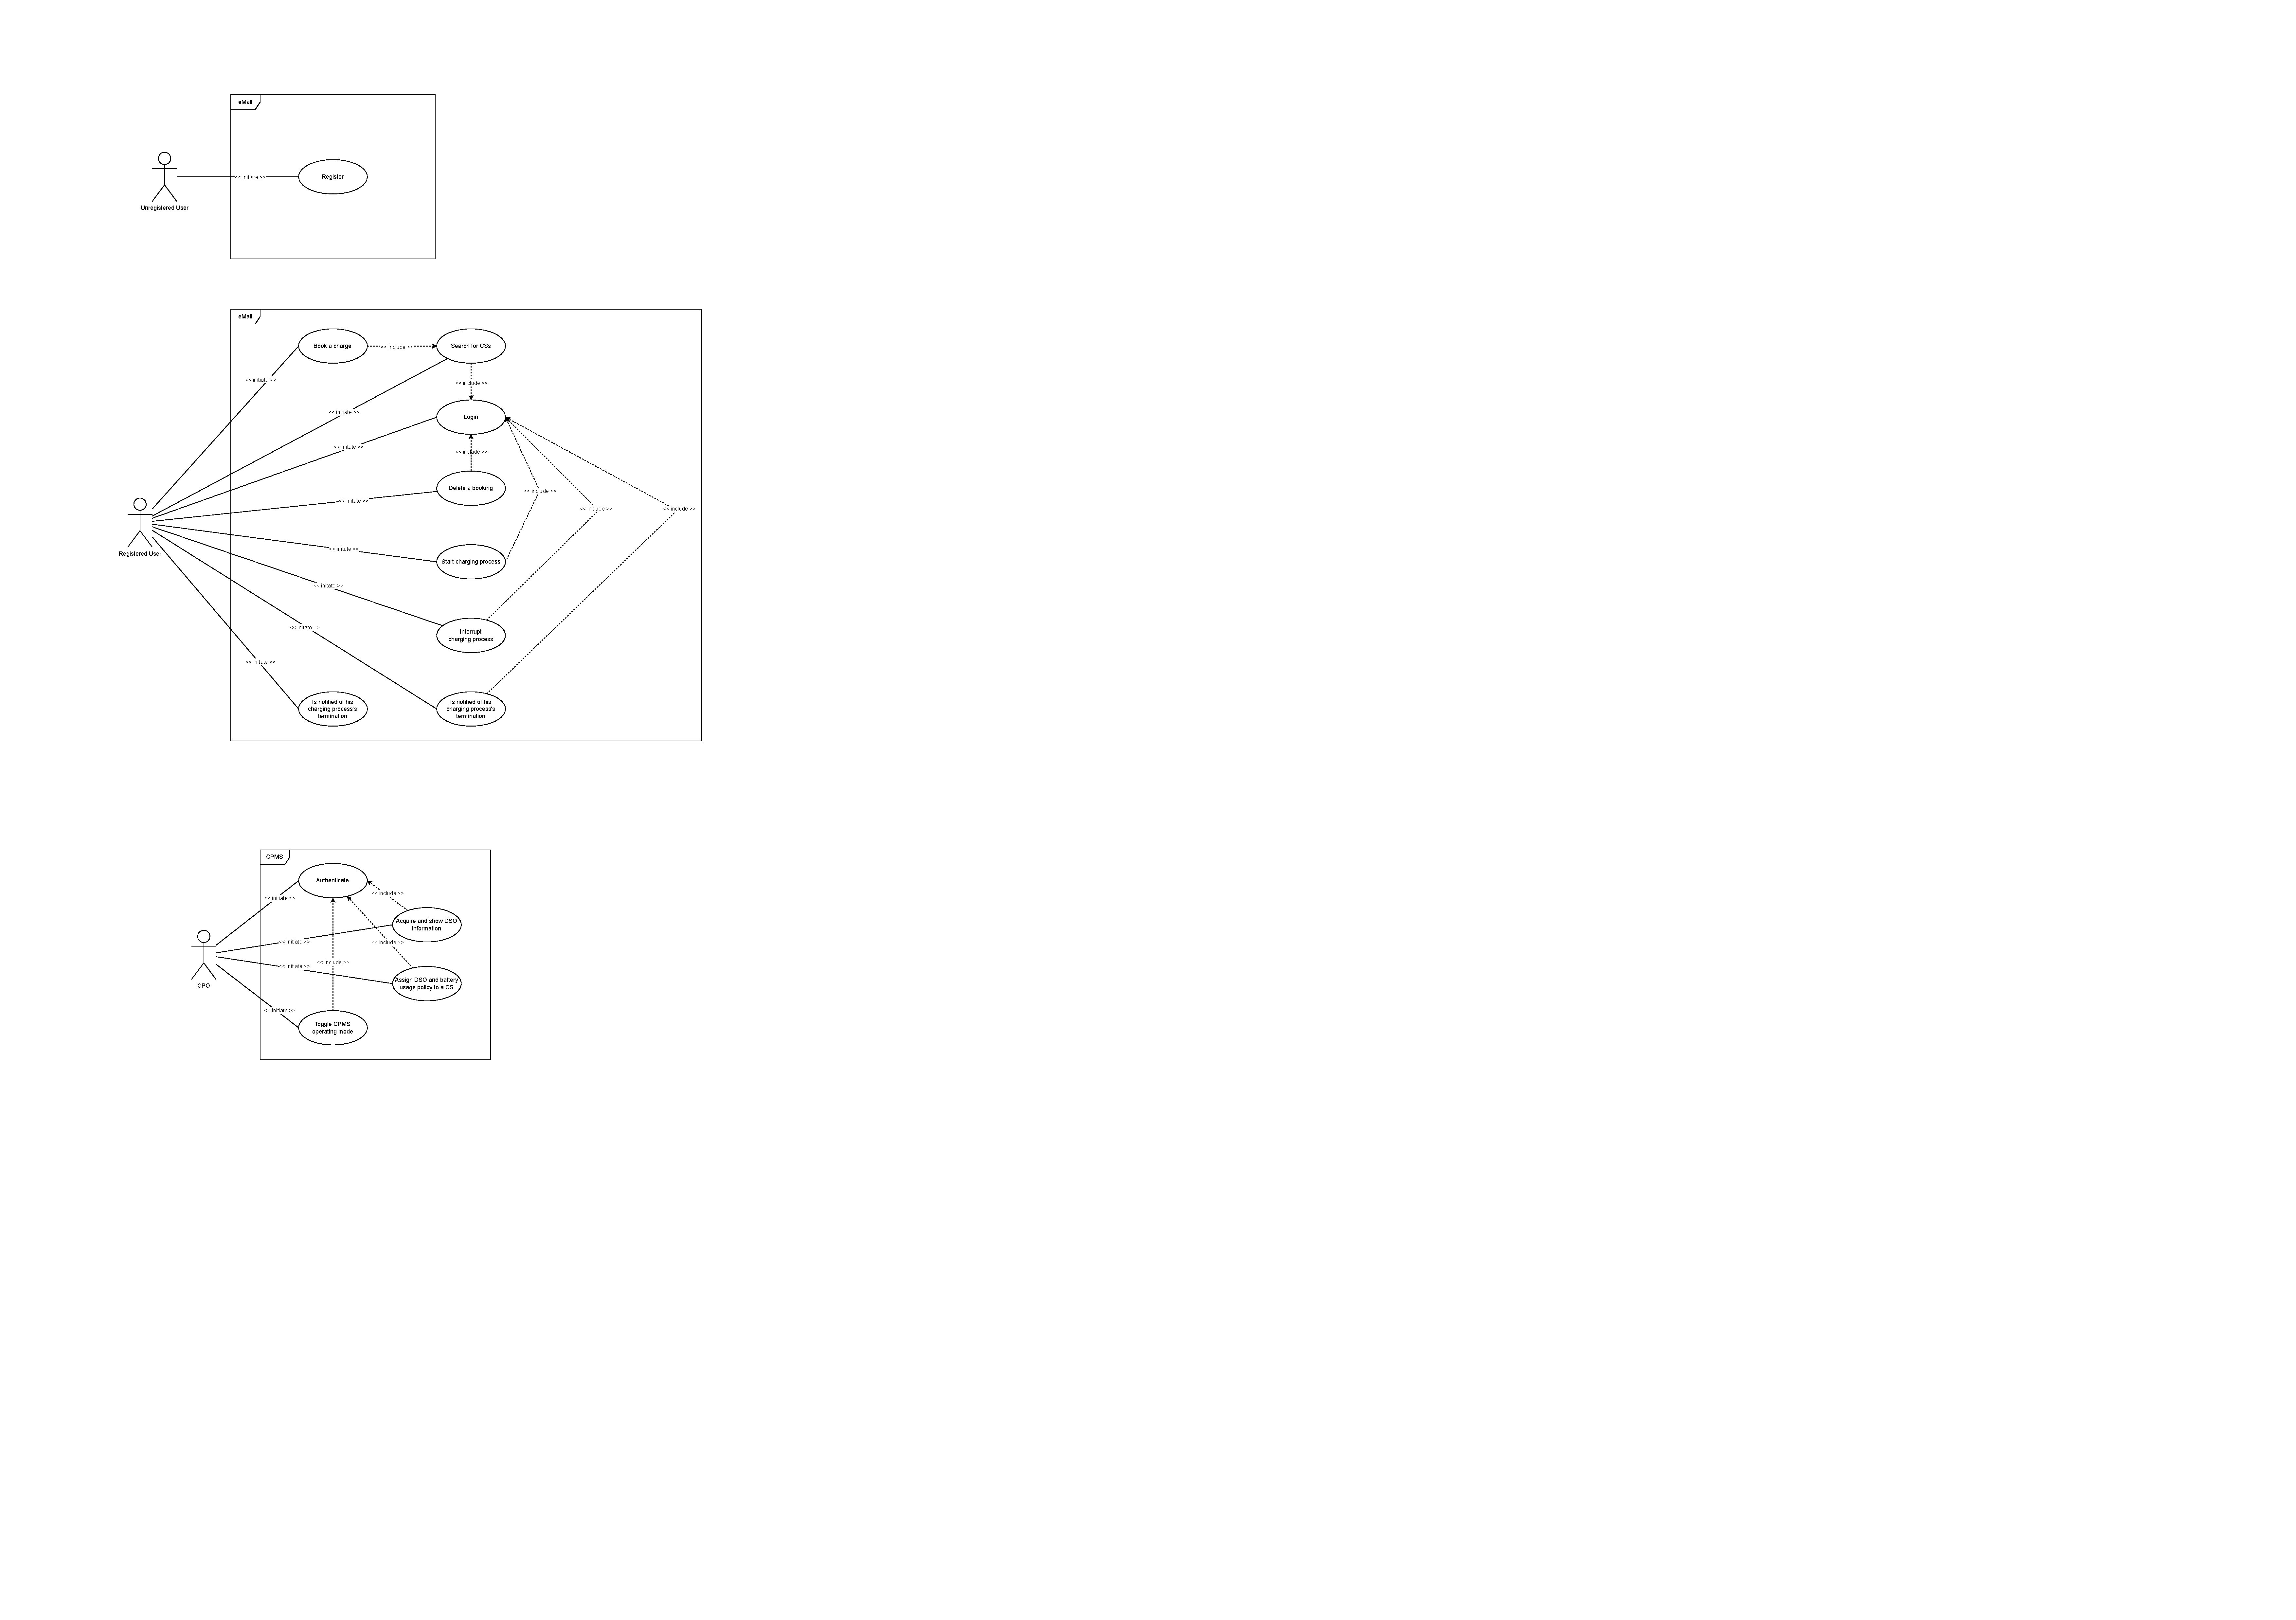
\includegraphics[page={1}, trim=7cm 9.7cm 7cm 9.6cm, width=0.6\linewidth, clip]{UseCases.pdf}
        \caption{Unregistered User}
    \end{figure}
    
    \item \textbf{2. Registered User}
    %trim = left bottom right top
    \begin{figure}[!ht]
        \centering
        \includegraphics[page={2}, trim=0cm 2.8cm 0cm 2.7cm, width=\linewidth, clip]{UseCases.pdf}
        \caption{Registered User}
    \end{figure}
    
    \item \textbf{3. CPO}
    %trim = left bottom right top
    \begin{figure}[!ht]
        \centering
        \includegraphics[page={3}, trim=6.6cm 8.8cm 6.6cm 8.8cm, width=0.8\linewidth, clip]{UseCases.pdf}
        \caption{CPO}
    \end{figure}
\end{description}

\newpage

\subsubsection{Sequence diagrams}

Here are the sequence diagrams corresponding one-to-one with the use cases in the above section, the entry conditins hold for the diagrams as well, hence things like "login" are not repeated in every diagram.

\begin{description}
    \item \textbf{1. New user registration}
    %trim = left bottom right top
    \begin{figure}[!ht]
        \centering
        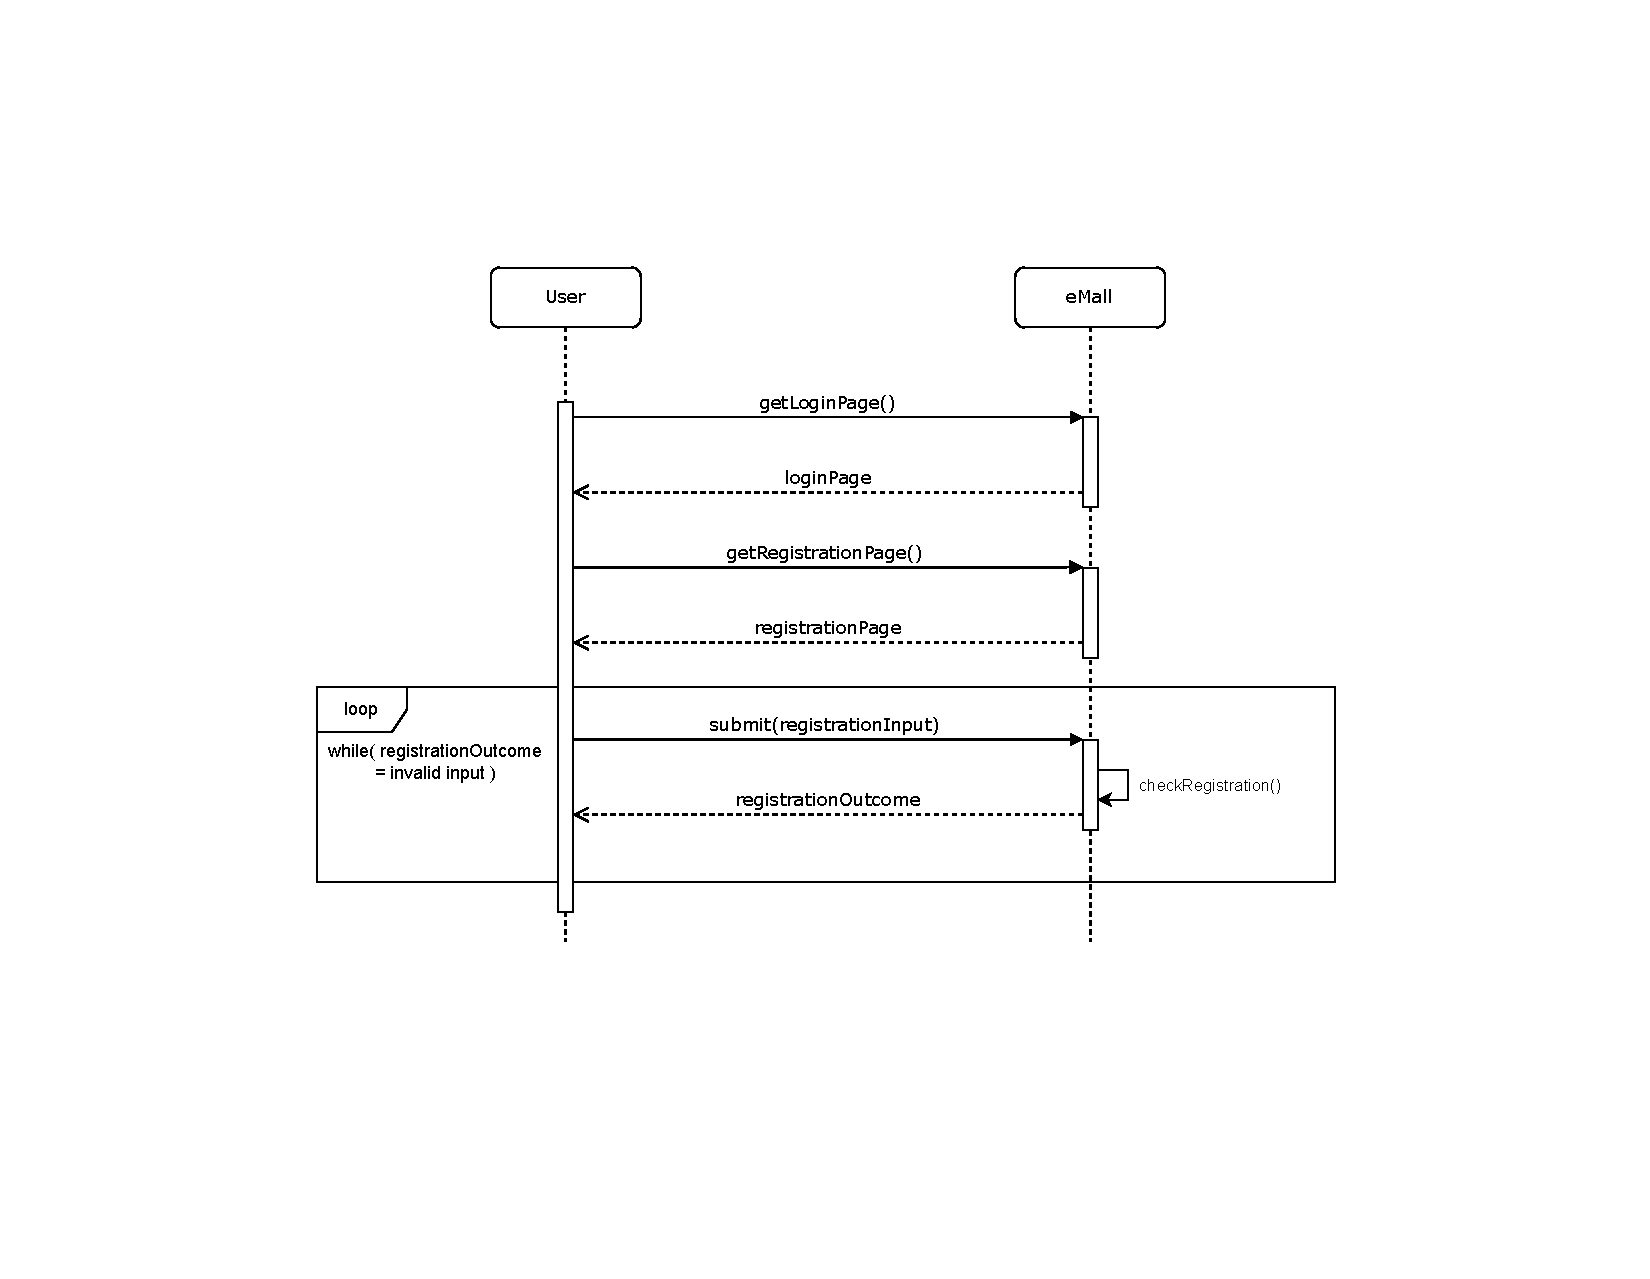
\includegraphics[page={1}, trim=5cm 5.6cm 5cm 4.4cm, width=0.8\linewidth, clip]{SequenceDiagrams.pdf}
        \caption{New user registration}
    \end{figure}
    
    \newpage
    
    \item \textbf{2. User login}
    %trim = left bottom right top
    \begin{figure}[!ht]
        \centering
        \includegraphics[page={2}, trim=5cm 9cm 5cm 3.6cm, width=0.8\linewidth, clip]{SequenceDiagrams.pdf}
        \caption{User login}
    \end{figure}
    
    \item \textbf{3. User searching and booking a CS}
    %trim = left bottom right top
    \begin{figure}[!ht]
        \centering
        \includegraphics[page={3}, trim=1.3cm 1.5cm 1.3cm 3cm, width=\linewidth, clip]{SequenceDiagrams.pdf}
        \caption{User searching and booking a CS}
    \end{figure}
    
    \item \textbf{4. User deleting one of his bookings}
    %trim = left bottom right top
    \begin{figure}[!ht]
        \centering
        \includegraphics[page={4}, trim=7cm 8cm 6cm 3cm, width=0.8\linewidth, clip]{SequenceDiagrams.pdf}
        \caption{User deleting one of his bookings}
    \end{figure}
    
    \item \textbf{5. User starting a charging process}
    %trim = left bottom right top
    \begin{figure}[!ht]
        \centering
        \includegraphics[page={5}, trim=1cm 8cm 0.5cm 2cm, width=\linewidth, clip]{SequenceDiagrams.pdf}
        \caption{User starting a charging process}
    \end{figure}
    
    \newpage
    
    \item \textbf{6. User interrupting a charging process}
    %trim = left bottom right top
    \begin{figure}[!ht]
        \centering
        \includegraphics[page={6}, trim=1cm 6.5cm 0.5cm 2cm, width=\linewidth, clip]{SequenceDiagrams.pdf}
        \caption{User interrupting a charging process}
    \end{figure}
    
    \item \textbf{7. Charging procedure self-terminates and User receives a notification}
    %trim = left bottom right top
    \begin{figure}[!ht]
        \centering
        \includegraphics[page={7}, trim=1cm 11cm 0.2cm 3cm, width=\linewidth, clip]{SequenceDiagrams.pdf}
        \caption{Charging procedure self-terminates and User receives a notification}
    \end{figure}
    
    \item \textbf{8. User does not show up for a booked recharge}
    %trim = left bottom right top
    \begin{figure}[!ht]
        \centering
        \includegraphics[page={8}, trim=11cm 12.3cm 8cm 4cm, width=0.3\linewidth, clip]{SequenceDiagrams.pdf}
        \caption{User does not show up for a booked recharge}
    \end{figure}
    
    \item \textbf{9. CPO requests information on DSOs’ energy prices and mix of sources}
    %trim = left bottom right top
    \begin{figure}[!ht]
        \centering
        \includegraphics[page={9}, trim=1cm 6.8cm 1.5cm 2.5cm, width=0.9\linewidth, clip]{SequenceDiagrams.pdf}
        \caption{CPO requests information on DSOs’ energy prices and mix of sources}
    \end{figure}
    
    \item \textbf{10. CPO assigns nominal-price, user-price, energy sources and battery usage policies for a CS}
    %trim = left bottom right top
    \begin{figure}[!ht]
        \centering
        \includegraphics[page={10}, trim=1cm 1.5cm 1cm 2.5cm, width=0.9\linewidth, clip]{SequenceDiagrams.pdf}
        \caption{CPO assigns nominal-price, user-price, energy sources and battery usage policies for a CS}
    \end{figure}
    
    \item \textbf{11. CPO toggles the CPMS operating mode}
    %trim = left bottom right top
    \begin{figure}[!ht]
        \centering
        \includegraphics[page={11}, trim=5cm 9cm 5.7cm 3.5cm, width=0.8\linewidth, clip]{SequenceDiagrams.pdf}
        \caption{CPO toggles the CPMS operating mode}
    \end{figure}
\end{description}

\subsubsection{Mapping on requirements}

\begin{table}[H]
    \centering
    %space between text and right/left borders
    \setlength{\tabcolsep}{18pt}
    %Row height multiplier
    \renewcommand{\arraystretch}{1.2}
    \begin{tabularx}{\textwidth}{|>{\hsize=1.2\hsize}X|>{\hsize=0.8\hsize}X|}
        \hline
        \textbf{Use case} & \textbf{Requirements} \\
        \hline
        ... & ... \\
        \hline
    \end{tabularx}
    \label{tab:useCasesMapping}
\end{table}

\subsection{Performance Requirements}
% LO METTIAMO IN TABELLA (VEDI COMMENTI CAMILLI)????
The system should be able to handle concurrent users, who may want to book or start a recharge at the same time in different geographical locations. As such, the systems should be capable of handling a reasonably high number of concurrent users, which we hypothesize to be in the order of 10.000. \\
Secondly, the system should operate with reasonable response times (of max 5 seconds), necessary to provide timely feedback to users who are booking or paying for a recharge, as well as users who want to start their recharge quickly. \\
Finally, the system should work properly even when accessed from a low-speed connectivity, such as 3G networks, since it is expected that users who might want to start a recharge through the system are probably going to access it through their mobile phone. As such, the overall amount of data exchanged with the user should be kept at a minimum. \\

\subsection{Design Constraints}
\subsubsection{Standards compliance}
The system should adhere to the standards and regulations imposed by the GDPR privacy law, since it is expected to be deployed (entirely or partially) in European countries. \\
Secondly, the APIs used for communications between the eMSP and CPMSs, as well as APIs used to share data between other parties in the STB should follow the current industry standard for API design which, at the time of writing, is the REST architecture. \\
Finally, the STB should function as expected on all modern web browser, without loss of functionalities according to the browser chosen by the user. 

\subsubsection{Hardware limitations}
Given that the system will be accessed from the Web and will require a connection to the platform to carry out its functions, the hardware must support some form of Internet connectivity (such as Wi-Fi, Ethernet or Cellular) and must have at least one modern Browser installed. \\
Furthermore, given that it is expected that the STB is mostly going to be accessed on mobile devices, it should not require a high processing power in order to perform its front-end functions. \\

\subsubsection{Any other constraint}

\subsection{Software System Attributes}
%Io prendo il treno, ciao, a domani!
%OK a domani!
\subsubsection{Reliability}
The system should be highly reliable and be up and running most of the times, since without it the user would not be able to start a recharge previously booked by the system. Hence regular maintenance is expected, together with some precautions that help reduce the risk of total outages in case of failures (e.g. geographical redundancy).

\subsubsection{Availability}
High availability is crucial for this system for 2 main reasons:
\begin{itemize}
    \item Its entire business model is based off of transactions made through the system (users booking and, later, paying for recharges)
    \item Users need the system to be up and running in order to start a recharge, even if it was already booked
\end{itemize}
Taking this into consideration, it is deemed appropriate to have an availability of 99.99\%, which would result in a maximum of approximately 52 minutes of downtime in an entire year. To achieve such a high figure, it may be essential to run components in parallel, making use of redundant machines and databases. \\
Furthermore, since the system also relies on external components (including, but not limited to the systems owned by DSOs), it should be noted that these systems may have lower availability constraints, and as such our STB should not fail entirely due to the failure of such dependencies.

\subsubsection{Security}
Since the STB has to deal with highly confidential user data (including, but not limited to billing information), the latest security standards should be applied. In practice, this boils down to the adoption of secure protocols for transferring information over the Internet (e.g. HTTPS), actively checking the authorization status of a user when they attempt to access a resource or a specific endpoint, as well as proper encryption of passwords when stored into the system.
%RIFRASARE O TOGLIERE????
Prevent an asshole to create 1 trillion accounts and occupy all of a city worth of CS, hence require credit card info on registration!

\subsubsection{Maintainability}
The system should be easily maintainable, to allow for future expansion of its feature set without requiring to build it from scratch. As such, standard software patterns should be adopted, and the whole architecture and underlying code should be properly and extensively documented, to allow potential future developers to start working on it without reading the entire code base.

\subsubsection{Portability}
As mentioned in previous sections, the system should be accessible both on a Desktop browser and on Mobile ones, therefore its interface should be fully responsive to adapt to different screen sizes. Futhermore, the system should be able to run on a wide variety of modern browsers, without feature restrictions for some of them.

\newpage

\section{Formal Analysis Using Alloy}
\label{section:alloy}

Follows a formal analysis of the system discussed in this document using Alloy, a formal language used to specify software models. This aims to prove that the model's constraints are satisfiable by instances that allow for the goals of the system to be archived.\\
\\
All classes modelled in the \hyperref[subsection:classDiagram]{\textbf{class diagram}} are present in this model as \textit{signatures}, together with those attributes that were deemed better modelled by dedicated \textit{signatures} rather than basic types. Note that the representation of time used within \textit{Date} is the same as the Unix Time, and the \textit{Now} signature is randomly chosen during the evaluation of the model to represent the current time. \\
\\
The present \textit{facts} model the impact of requirements on the model, while \textit{predicates} allow for the \hyperref[subsec:prodfunctions]{\textbf{product functions}} previously described. \\

%\bgroup\obeylines \code{
%    This is alloy
%}
%\egroup

\begin{ffcode}
    sig Date {
	unixTime: one Int
    } {
    	unixTime >= 0
    }
    //Radomly chosen by Alloy
    one sig Now extends Date {}
    
    sig Location {}
    sig Email {}
    sig UserName {}
    sig Password {}
    sig CompanyName {}
    sig PaymentMethod {}
    
    abstract sig Bool {}
    one sig True extends Bool {}
    one sig False extends Bool {}
    
    sig User {
    	userName: one UserName,
    	email: one Email,
    	password: one Password,
    	paymentMethod: one PaymentMethod,
    	bookings: set Booking
    } {
    	//No user can have two overlapping bookings
    	all b1, b2: Booking | (b1 in bookings and b2 in bookings)
    	implies
    	(b1 = b2 or (b1.startDate.unixTime < b2.startDate.unixTime and b1.endDate.unixTime <= b2.startDate.unixTime) or
    	(b2.startDate.unixTime < b1.startDate.unixTime and b2.endDate.unixTime <= b1.startDate.unixTime))
    }
    
    //Force that a booking of a eMSP is made by a user registered in that eMSP, even tho the eMSP is only one...
    sig Booking {
    	startDate: one Date,
    	endDate: one Date,
    	isActive: one Bool,
    	socket: one Socket
    } {
    	startDate.unixTime < endDate.unixTime
    	and (isActive = True implies startDate.unixTime <= Now.unixTime and Now.unixTime <= endDate.unixTime)
    	and (isActive = True implies socket.connectedVehicle != none)
    }
    
    //For our interests, it is a singleton
    one sig eMSP {
    	users: some User,
    	knownCPMSs: some CPMS,
    	bookings: some Booking
    }
    
    //The CS->CPO one-to-one relation can be inferred by going through here
    sig CPMS {
    	CSs: some CS,
    	knownDSOs: some DSO,
    	owner: one CPO,
    	policy: one Policy
    }
    
    sig Policy {
    	weights: set Int,
    	thresholds: set Int
    } {
    	all w: Int | w in weights implies w >= 0
    	and all t: Int | t in thresholds implies t >= 0
    }
    
    sig CS {
    	//Do we really need socketCount?
    	socketCount: one Int,
    	location: one Location,
    	nominalPrice: one Int,
    	userPrice: one Int,
    	chargingFromBatteries: one Bool,
    	sockets: some Socket,
    	batteries: set Battery,
    	currentDSO: one DSO
    } {
    	socketCount > 0
    	and nominalPrice > 0
    	and userPrice > 0
    	and userPrice <= nominalPrice
    	and nominalPrice >= currentDSO.price
    }
    
    sig Connector {}
    
    sig Socket {
    	connector: one Connector,
    	maxPower: one Int,
    	currentPower: one Int,
    	connectedVehicle: lone Vehicle
    } {
    	maxPower > 0
    	and currentPower >= 0
    	and currentPower <= maxPower
    }
    
    sig Vehicle {
    	chargePerc: one Int
    } {
    	chargePerc >= 0 and chargePerc <= 10
    }
    
    sig CPO {
    	name: one CompanyName
    }
    
    sig DSO {
    	name: one CompanyName,
    	price: one Int,
    	energyMix: one EnergyMix
    } {
    	price > 0
    }
    
    sig EnergyMix {
    	oilAndGas: Int,
    	ccgt: Int,
    	coal: Int,
    	nuclear: Int,
    	hydroelectric: Int,
    	otherRenewableSources: Int
    } {
    	//The sum will need to reach 100 in reality, but here we are working with 4-bit integers
    	oilAndGas + ccgt + coal + nuclear + hydroelectric + otherRenewableSources = 10
    	and oilAndGas >= 0
    	and ccgt >= 0
    	and coal >= 0
    	and nuclear >= 0
    	and hydroelectric >= 0
    	and otherRenewableSources >= 0
    }
    
    sig Battery {
    	capacitymAp: one Int,
    	chargeLevel: one Int
    } {
    	capacitymAp > 0 and
    	chargeLevel >= 0 and chargeLevel <= 10
    }
    
    fact noCPOsWithSameName {
    	no c1, c2: CPO | c1 != c2 and c1.name = c2.name
    }
    
    fact noDSOWIthSameName {
    	no d1, d2: DSO | d1 != d2 and d1.name = d2.name
    }
    
    fact noCPODSOWithSameName {
    	no c: CPO, d: DSO | c.name = d.name
    }
    
    fact CPOOneToOneCPMS {
    	no cp1, cp2: CPMS | cp1 != cp2 and cp1.owner = cp2.owner
    }
    
    fact noBookingsWithoutUsers {
    	all b: Booking | (one u: User | b in u.bookings)
    }
    
    fact noExpiredBookings {
    	all b: Booking | b.endDate.unixTime >= Now.unixTime
    }
    
    fact noOverlappingSocketBookings {
    	/*
    	or ((b1.startDate.unixTime < b2.startDate.unixTime implies b1.endDate.unixTime <= b2.startDate.unixTime) and (b1.startDate.unixTime > b2.startDate.unixTime implies b2.endDate.unixTime <= b1.startDate.unixTime))
    	*/
    	all b1, b2: Booking | (b1 = b2 or b1.socket != b2.socket or (b1.startDate.unixTime < b2.startDate.unixTime and b1.endDate.unixTime <= b2.startDate.unixTime)
    	or (b2.startDate.unixTime < b1.startDate.unixTime and b2.endDate.unixTime <= b1.startDate.unixTime))
    }
    
    fact socketFreeIfNotBooked {
    	all s: Socket | ((no b: Booking | b.socket = s)
    	implies 
    	no s.connectedVehicle)
    }
    
    fact socketNotFreeIfActiveBooking {
    	all s: Socket | ((some b: Booking | b.socket = s and b.isActive = True)
    	implies 
    	s.connectedVehicle != none)
    }
    
    fact allCSHaveACPMS {
    	//no cs: CS | (no cpm: CPMS | (cs in cpm.CSs))
    	all cs: CS | (one cpm: CPMS | cs in cpm.CSs)
    }
    
    fact uniqueSocketsForCS {
    	no cs1, cs2: CS | cs1 != cs2 and (some s: Socket | s in cs1.sockets and s in cs2.sockets)
    }
    
    run {} for 12 but 6 Int, exactly 3 User, exactly 3 CS, exactly 2 CPMS, exactly 3 Booking
    
\end{ffcode}

\newpage

\section{Effort Spent}
\label{section:effort}

\subsection{Ronzani Marco - mat: 224578}

\begin{tabular}{|l|l|}
    \hline
    \textbf{Task} & \textbf{Time spent} \\
    \hline
    Introduction & $10\ h$ \\
    \hline
    Overall Description & $15\ h$ \\
    \hline
    Specific Requirements & $14\ h$ \\
    \hline
    Formal Analysis & $6\ h$ \\
    \hline
    Other & $3\ h$ \\
    \hline
    \hline
    Total & $48 h$ \\
    \hline
\end{tabular}

\subsection{Sassi Alessandro - mat: ...}

\begin{tabular}{|l|l|}
    \hline
    \textbf{Task} & \textbf{Time spent} \\
    \hline
    Introduction & $\infty h$ \\
    \hline
    Overall Description & $\infty h$ \\
    \hline
    Specific Requirements & $\infty h$ \\
    \hline
    Formal Analysis & $\infty h$ \\
    \hline
    Other & $\infty h$ \\
    \hline
    \hline
    Total & $5*\infty h$ \\
    \hline
\end{tabular}

\section{References}
\label{section:references}

\begin{enumerate}
    \item \href{https://www.platformelectromobility.eu/2022/05/17/ev-charging-how-to-tap-in-the-grid-smartly/}{Platform for Electromobility. EV Charging: How to tap in the grid smartly?}.
    \item \href{https://mobilityintegrationsymposium.org/wp-content/uploads/sites/10/2018/11/4A_3_Emob18_024_paper_Filipe_Campos.pdf}{F. Campos, L. Marques, and K. Kotsalos, Electric Vehicle CPMS and Secondary Substation Management}.
    \item \href{https://doi.org/10.1145/3297067.3297078}{Shu Su, Hui Yan, and Ning Ding. 2018. Machine Learning-Based Charging Network Operation Service Platform Reservation Charging Service System. In Proceedings of the 2018 International Conference on Signal Processing and Machine Learning (SPML '18). Association for Computing Machinery, New York, NY, USA, 1–5}.
    \item Jan Mrkos, Antonín Komenda, and Michal Jakob. 2018. Revenue Maximization for Electric Vehicle Charging Service Providers Using Sequential Dynamic Pricing. In Proceedings of the 17th International Conference on Autonomous Agents and MultiAgent Systems (AAMAS '18). International Foundation for Autonomous Agents and Multiagent Systems, Richland, SC, 832–840.
\end{enumerate}

\end{document}